%===============================================================================
% LaTeX sjabloon voor de bachelorproef toegepaste informatica aan HOGENT
% Meer info op https://github.com/HoGentTIN/latex-hogent-report
%===============================================================================

\documentclass[dutch,dit,thesis]{hogentreport}

% TODO:
% - If necessary, replace the option `dit`' with your own department!
%   Valid entries are dbo, dbt, dgz, dit, dlo, dog, dsa, soa
% - If you write your thesis in English (remark: only possible after getting
%   explicit approval!), remove the option "dutch," or replace with "english".

\usepackage{lipsum} % For blind text, can be removed after adding actual content
\usepackage{listings}
\usepackage{xcolor} % Voor kleurondersteuning
\usepackage{tikz} 


%% Pictures to include in the text can be put in the graphics/ folder
\graphicspath{{../graphics/}}

%% For source code highlighting, requires pygments to be installed
%% Compile with the -shell-escape flag!
%% \usepackage[chapter]{minted}
%% If you compile with the make_thesis.{bat,sh} script, use the following
%% import instead:
\usepackage[chapter,outputdir=../output]{minted}
\usemintedstyle{solarized-light}

%% Formatting for minted environments.
\setminted{%
    autogobble,
    frame=lines,
    breaklines,
    linenos,
    tabsize=4
}

%% Ensure the list of listings is in the table of contents
\renewcommand\listoflistingscaption{%
    \IfLanguageName{dutch}{Lijst van codefragmenten}{List of listings}
}
\renewcommand\listingscaption{%
    \IfLanguageName{dutch}{Codefragment}{Listing}
}
\renewcommand*\listoflistings{%
    \cleardoublepage\phantomsection\addcontentsline{toc}{chapter}{\listoflistingscaption}%
    \listof{listing}{\listoflistingscaption}%
}

% Other packages not already included can be imported here

%%---------- Document metadata -------------------------------------------------
% TODO: Replace this with your own information
\author{Lucas Van Compernolle}
\supervisor{Dhr. J. Courtens}
\cosupervisor{Dhr. W. Lahousse}
\title[]%
    {Modernisering van Messaging Systeem tussen PLC en WMS: Een Onderzoek naar efficiëntie, betrouwbaarheid en performantie}
\academicyear{\advance\year by -1 \the\year--\advance\year by 1 \the\year}
\examperiod{1}
\degreesought{\IfLanguageName{dutch}{Professionele bachelor in de toegepaste informatica}{Bachelor of applied computer science}}
\partialthesis{false} %% To display 'in partial fulfilment'
%\institution{Internshipcompany BVBA.}

%% Add global exceptions to the hyphenation here
\hyphenation{back-slash}

%% The bibliography (style and settings are  found in hogentthesis.cls)
\addbibresource{bachproef.bib}            %% Bibliography file
\addbibresource{../voorstel/voorstel.bib} %% Bibliography research proposal
\defbibheading{bibempty}{}

%% Prevent empty pages for right-handed chapter starts in twoside mode
\renewcommand{\cleardoublepage}{\clearpage}

\renewcommand{\arraystretch}{1.2}

%% Content starts here.

\begin{document}

%---------- Front matter -------------------------------------------------------

\frontmatter

\hypersetup{pageanchor=false} %% Disable page numbering references
%% Render a Dutch outer title page if the main language is English
\IfLanguageName{english}{%
    %% If necessary, information can be changed here
    \degreesought{Professionele Bachelor toegepaste informatica}%
    \begin{otherlanguage}{dutch}%
       \maketitle%
    \end{otherlanguage}%
}{}

%% Generates title page content
\maketitle
\hypersetup{pageanchor=true}

%%=============================================================================
%% Voorwoord
%%=============================================================================

\chapter*{\IfLanguageName{dutch}{Woord vooraf}{Preface}}%
\label{ch:voorwoord}

%% TODO:
%% Het voorwoord is het enige deel van de bachelorproef waar je vanuit je
%% eigen standpunt (``ik-vorm'') mag schrijven. Je kan hier bv. motiveren
%% waarom jij het onderwerp wil bespreken.
%% Vergeet ook niet te bedanken wie je geholpen/gesteund/... heeft

Omdat ik een grote interesse heb in de technologie dat de werking met andere 
applicaties mogelijk maakt, heb ik dit onderwerp gekozen.
Het leerde mij om met een andere perceptie te kijken naar de werking van een systeem. De non-functionele kant van de werking tussen twee services.
\newline

Ik bedankt mijn promotor voor de steun in het halen van deadlines, 
de kalmte en het vertrouwen die hij me gaf in het succesvol afronden van dit traject.
Daarnaast bedankt ik ook mijn co-promotor die me geholpen heeft om dit onderwerp aan te pakken binnen het bedrijf.
Als laatste bedankt ik TVH, die me altijd geholpen heeft in mijn persoonlijke groei.
%%=============================================================================
%% Samenvatting
%%=============================================================================

% TODO: De "abstract" of samenvatting is een kernachtige (~ 1 blz. voor een
% thesis) synthese van het document.
%
% Een goede abstract biedt een kernachtig antwoord op volgende vragen:
%
% 1. Waarover gaat de bachelorproef?
% 2. Waarom heb je er over geschreven?
% 3. Hoe heb je het onderzoek uitgevoerd?
% 4. Wat waren de resultaten? Wat blijkt uit je onderzoek?
% 5. Wat betekenen je resultaten? Wat is de relevantie voor het werkveld?
%
% Daarom bestaat een abstract uit volgende componenten:
%
% - inleiding + kaderen thema
% - probleemstelling
% - (centrale) onderzoeksvraag
% - onderzoeksdoelstelling
% - methodologie
% - resultaten (beperk tot de belangrijkste, relevant voor de onderzoeksvraag)
% - conclusies, aanbevelingen, beperkingen
%
% LET OP! Een samenvatting is GEEN voorwoord!

%%---------- Nederlandse samenvatting -----------------------------------------
%
% TODO: Als je je bachelorproef in het Engels schrijft, moet je eerst een
% Nederlandse samenvatting invoegen. Haal daarvoor onderstaande code uit
% commentaar.
% Wie zijn bachelorproef in het Nederlands schrijft, kan dit negeren, de inhoud
% wordt niet in het document ingevoegd.

\IfLanguageName{english}{%
\selectlanguage{dutch}
\chapter*{Samenvatting}
% \lipsum[1-4]



\selectlanguage{english}
}{}

%%---------- Samenvatting -----------------------------------------------------
% De samenvatting in de hoofdtaal van het document

\chapter*{\IfLanguageName{dutch}{Samenvatting}{Abstract}}

% \lipsum[1-4]

% Intro (use case doelpubliek en doelstelling) 
% Kaderen thema
Dit onderzoek situeert zich binnen de IT afdeling van TVH (Thermote \& Vanhalst). 
TVH is een bedrijf met als hoofdactiviteit het verkopen van onderdelen in de logistieke sector.
Het bedrijf bestaat uit meerdere automatische magazijnen die instaan voor de opslag van goederen. 
Een automatisch magazijn bestaat uit meerdere IT componenten genaamd services, die elk hun specifieke verantwoordelijkheden hebben. 
Om de gehele werking te kunnen garanderen moeten deze componenten met elkaar kunnen communiceren. 
\newline

% Probleemstelling
De huidige Unix-server die instaat voor de communicatie, maakt gebruik van \mbox{CentOS} als besturingssysteem,
wordt niet ondersteund en is verouderd.
Hierdoor is de server onderhevig aan veiligheidsrisico's en moet die vervangen worden door een server met een Redhat OS, 
die wel officiële ondersteuning aanbiedt.
De gebruikte messaging software, SonicMQ, is eveneens verouderd en kan niet geïnstalleerd worden op de nieuwe server. 
\newline

Omdat vervanging noodzakelijk is, is de vraag in dit onderzoek: 
Welke modern messaging systeem kan het huidige SonicMQ-systeem tussen de PLC en het WMS vervangen, 
met aandacht voor compatibiliteit, efficiëntie, betrouwbaarheid, veiligheid en kosten?
Deze vraag vormt de leidraad voor het onderzoek met als doel 
% doel
het SonicMQ messaging-systeem te vervangen door een moderner, future-proof systeem.
Naast de integratie van de nieuwe software, moet deze ook voldoen aan de vereisten
om de continuïteit van het automatische magazijn te waarborgen. 
Daarom is dit onderzoek nodig om de meest geschikte technologieën te identificeren met als doel de optimale oplossing te adviseren.
\newline

% Opbouw paper
Om een duidelijk overzicht te bieden zal deze paper eerst dieper ingaan op de kernbegrippen 
om de context te verduidelijken waarin de bachelorproef wordt uitgevoerd.
\newline

% Methode
Om een doordachte keuze te kunnen maken, worden verschillende messaging-systemen onderzocht en vergeleken.
Hiervoor is een shortlist opgesteld waarin elke technologie wordt geëvalueerd.
De geselecteerde technologieën worden aan verschillende testen onderworpen in een virtuele omgeving die de communicatie van het automatische magazijn simuleert. 
Op deze manier kan een weloverwogen keuze worden gemaakt die voldoet aan de non-functional requirements.

%---------- Inhoud, lijst figuren, ... -----------------------------------------

\tableofcontents

% In a list of figures, the complete caption will be included. To prevent this,
% ALWAYS add a short description in the caption!
%
%  \caption[short description]{elaborate description}
%
% If you do, only the short description will be used in the list of figures

\listoffigures

% If you included tables and/or source code listings, uncomment the appropriate
% lines.
\listoftables

\listoflistings

% Als je een lijst van afkortingen of termen wil toevoegen, dan hoort die
% hier thuis. Gebruik bijvoorbeeld de ``glossaries'' package.
% https://www.overleaf.com/learn/latex/Glossaries

%---------- Kern ---------------------------------------------------------------

\mainmatter{}

% De eerste hoofdstukken van een bachelorproef zijn meestal een inleiding op
% het onderwerp, literatuurstudie en verantwoording methodologie.
% Aarzel niet om een meer beschrijvende titel aan deze hoofdstukken te geven of
% om bijvoorbeeld de inleiding en/of stand van zaken over meerdere hoofdstukken
% te verspreiden!

%%=============================================================================
%% Inleiding
%%=============================================================================

\chapter{\IfLanguageName{dutch}{Inleiding}{Introduction}}%
\label{ch:inleiding}

% De inleiding moet de lezer net genoeg informatie verschaffen om het onderwerp te begrijpen en in te zien waarom 
% de onderzoeksvraag de moeite waard is om te onderzoeken. 
% In de inleiding ga je literatuurverwijzingen beperken, zodat de tekst vlot leesbaar blijft. 
% Je kan de inleiding verder onderverdelen in secties als dit de tekst verduidelijkt. 
% Zaken die aan bod kunnen komen in de inleiding~\autocite{Pollefliet2011}:

% \begin{itemize}
%   \item Context
%   \item Het onderwerp
%   \item Verantwoording van het onderwerp, methodologie
%   \item Probleemstelling
%   \item Onderzoeksdoelstelling
%   \item Onderzoeksvraag
%   \item \ldots
% \end{itemize}

\section{\IfLanguageName{dutch}{Context}{Context}}%
\label{sec:context}
% Context
TVH is een retail bedrijf dat zich focust op de verkoop van onderdelen binnen de logistieke sector. 
Bedrijven zoals TVH hebben verschillende domeinen en subdomeinen met specifieke doeleinden binnen de organisatie. 
Deze bachelorproef speelt zich af binnen het domein "warehousing", dat instaat voor het beheer van goederen.
Warehousing in TVH bevat verschillende subcomponenten waaronder het WMS (Warehouse Management System) en WCS (Warehouse Control System).
Goederen kunnen naar een bepaalde bestemming in het gebouw getransporteerd worden via een transportband, genaamd conveyor.
Hiervoor is er communicatie nodig in beide richtingen tussen het WCS (Warehouse Control System) en de PLC's (Programmable Logic Controllers).
De PLC's voor het transportsysteem worden beheerd door techniekers van het automatisatie team.
Het WCS systeem, geschreven in Progress 4GL-code en de server die verantwoordelijk is voor de communicatie worden beheerd door IT.
\newline
\newpage

\section{\IfLanguageName{dutch}{Het onderwerp}{Het onderwerp}}%
\label{sec:Het onderwerp}
% Afbakening
% Server
Omdat het transportsysteem een van de eerste systemen is die werden geïmplementeerd, is het inmiddels verouderd. 
De server die verantwoordelijk is voor de communicatie draait op CentOS 6.6 en bied geen ondersteuning meer sinds 30 november 2020 ~\autocite{Reock2020}.
Vervanging door een modern systeem is noodzakelijk, aangezien de veiligheid in het gedrang komt.
Systemen die End of Life (EoL) zijn, ontvangen geen ondersteuning of updates meer van de leverancier, 
wat ze kwetsbaar maakt voor aanvallen.
Hackers kunnen dergelijke servers eenvoudig aanvallen omdat bekende kwetsbaarheden niet langer worden verholpen \autocite{Mittal2024}.
Het vervangen van de server zelf valt buiten de scope van dit onderzoek en zal worden overgedragen aan het IT-infrastructuurteam binnen het bedrijf
\begin{table}[h!]
  \centering
  \begin{tabular}{|c|c|c|}
      \hline
      \textbf{Version} & \textbf{Release Date} & \textbf{End-of-Life Date} \\
      \hline
      CentOS 8 & September 24, 2019 & December 31, 2021 \\
      \hline
      CentOS 7 & July 7, 2014 & June 30, 2024 \\
      \hline
      CentOS 6 & July 10, 2011 & November 30, 2020 \\
      \hline
      CentOS 5 & April 12, 2007 & March 31, 2017 \\
      \hline
  \end{tabular}
  \caption{CentOS Release and End-of-Life Dates~\autocite{Reock2020}}
  \label{tab:centos6}
\end{table}
\newline
 
% Software
De software op die server, SonicMQ 7.0 van Progress Software Corporation, werkt als de ``middleware'' voor de communicatie.
Omdat deze software verouderd is, niet meer ondersteund wordt en niet kan geïnstalleerd worden op een modern OS, moeten we zoeken naar een alternatief.
Dit onderzoek richt zich dan ook op het grondig onderzoeken en vergelijken van geschikte alternatieven die voldoen aan de 
niet-functionele eisen van het automatisch magazijn. Deze vereisten worden later toegelicht in het hoofdstuk methodologie.
\newline

\section{\IfLanguageName{dutch}{Probleemstelling}{Problem Statement}}%
\label{sec:Probleemstelling}

% Uit je probleemstelling moet duidelijk zijn dat je onderzoek een meerwaarde heeft voor een concrete doelgroep. De doelgroep moet goed gedefinieerd en afgelijnd zijn. 
% Doelgroepen als ``bedrijven,'' ``KMO's'', systeembeheerders, enz.~zijn nog te vaag. 
% Als je een lijstje kan maken van de personen/organisaties die een meerwaarde zullen vinden in deze bachelorproef (dit is eigenlijk je steekproefkader), 
% dan is dat een indicatie dat de doelgroep goed gedefinieerd is.
% Dit kan een enkel bedrijf zijn of zelfs één persoon (je co-promotor/opdrachtgever).

% Probleemstelling
Verouderde software is gevoelig voor uitval, kostelijk om te onderhouden en bevat extra complexiteit om te integreren met andere systemen.
Dit beïnvloedt de continuïteit en verhoogt de onderhoudskosten~\autocite{Khadka2016}.
Volgende nadelen van verouderde software doen zich voor: 
\begin{itemize}
  \item De onderhoudskosten, waardoor mensen in de firma specifiek opgeleid moeten worden om deze te onderhouden. 
  \item Beveilgingsrisico's, cybercriminelen richten zich vaak op verouderde software, omdat de kwetsbaarheden publiekelijk bekend zijn en niet meer worden aangepakt.
  \item Betrouwbaarheid, omdat verouderde software een hogere kans heeft op uitval, kan dit leiden tot hogere kosten door verlies van productiviteit en herstelwerkzaamheden.
\end{itemize}

Tijdens een uitval kan het systeem geen data meer versturen, noch ontvangen. 
Hierdoor kunnen bestellingen van klanten vertraging oplopen en kunnen dus de kosten hoog oplopen.
Vervanging van deze software is dus noodzakelijk, waardoor volgende vraag kan gesteld worden: 
\newline
\emph{Welke moderne messaging systeem kan het huidige SonicMQ-systeem tussen de PLC en het WMS vervangen, 
met aandacht voor compatibiliteit, efficiëntie, betrouwbaarheid, veiligheid en kosten?}
\newline

Deze vraag vormt de leidraad voor het onderzoek naar een nieuw systeem die toekomstbestendig is 
en de continuïteit van het automatische magazijn kan waarborgen.

 
\section{\IfLanguageName{dutch}{Onderzoeksvraag}{Research question}}%
\label{sec:Onderzoeksvraag}

% Wees zo concreet mogelijk bij het formuleren van je onderzoeksvraag. 
% Een onderzoeksvraag is trouwens iets waar nog niemand op dit moment een antwoord heeft (voor zover je kan nagaan). 
% Het opzoeken van bestaande informatie (bv. ``welke tools bestaan er voor deze toepassing?'') is dus geen onderzoeksvraag. 
% Je kan de onderzoeksvraag verder specifiëren in deelvragen. 
% Bv.~als je onderzoek gaat over performantiemetingen, dan 

Welke \emph{messaging technologieën} zijn het meest geschikt om het verouderde SonicMQ software te vervangen 
en de continuïteit van automatische magazijn te garanderen?
\newline

Enkele cruciale deelvragen met betrekking tot de hoofdvraag:
\begin{enumerate} 
  \item Wat zijn de non-functional requirements?
  \item Waarom is een weloverwogen keuze van essentieel belang?
  \item Welke messaging systemen zijn er beschikbaar?
  \item Wat is de inspanning om een gekozen technologie te implementeren?
  \item Welk messaging systeem is een weloverwogen keuze?
\end{enumerate}


\section{\IfLanguageName{dutch}{Onderzoeksdoelstelling}{Research objective}}%
\label{sec:Onderzoeksdoelstelling}

% Wat is het beoogde resultaat van je bachelorproef? Wat zijn de criteria voor succes? Beschrijf die zo concreet mogelijk. 
% Gaat het bv.\ om een proof-of-concept, een prototype, een verslag met aanbevelingen, een vergelijkende studie, enz.
% onderzoeksdoelstelling

Het doel van dit onderzoek is om te bepalen welk messaging systeem het meest geschikt is voor de vervanging van de huidige SonicMQ,
die gebruikt wordt voor de communicatie tussen WMS en PLC. 
Hierbij moet er rekening gehouden worden met de niet-functionele vereisten,
zoals flexibiliteit, performantie, beveiliging, integratiemogelijkheden en kosten.
Dit onderzoek zal resulteren in een rapport met aanbevelingen.

\section{\IfLanguageName{dutch}{Opzet van deze bachelorproef}{Structure of this bachelor thesis}}%
\label{sec:Opzet-bachelorproef}

% Het is gebruikelijk aan het einde van de inleiding een overzicht te
% geven van de opbouw van de rest van de tekst. Deze sectie bevat al een aanzet
% die je kan aanvullen/aanpassen in functie van je eigen tekst.

De rest van deze bachelorproef is als volgt opgebouwd:
\begin{enumerate}
  \item In Hoofdstuk~\ref{ch:stand-van-zaken} wordt een overzicht gegeven van de stand van zaken binnen het onderzoeksdomein, op basis van een literatuurstudie.
  \item In Hoofdstuk~\ref{ch:methodologie} wordt de methodologie toegelicht en worden de gebruikte onderzoekstechnieken besproken om een antwoord te kunnen formuleren op de onderzoeksvragen.
  % TODO: Vul hier aan voor je eigen hoofstukken, één of twee zinnen per hoofdstuk
  \begin{enumerate}
    \item Vul hier aan voor je eigen hoofstukken, één of twee zinnen per hoofdstuk
    \item \dots
  \end{enumerate}
  \item In Hoofdstuk~\ref{ch:conclusie}, tenslotte, wordt de conclusie gegeven en een antwoord geformuleerd op de onderzoeksvragen. Daarbij wordt ook een aanzet gegeven voor toekomstig onderzoek binnen dit domein.
\end{enumerate}

\chapter{\IfLanguageName{dutch}{Stand van zaken}{State of the art}}%
\label{ch:stand-van-zaken}

% Tip: Begin elk hoofdstuk met een paragraaf inleiding die beschrijft hoe
% dit hoofdstuk past binnen het geheel van de bachelorproef. Geef in het
% bijzonder aan wat de link is met het vorige en volgende hoofdstuk.

% Pas na deze inleidende paragraaf komt de eerste sectiehoofding.

% Dit hoofdstuk bevat je literatuurstudie. De inhoud gaat verder op de inleiding, maar zal het onderwerp van de bachelorproef *diepgaand* uitspitten. 
% De bedoeling is dat de lezer na lezing van dit hoofdstuk helemaal op de hoogte is van de huidige stand van zaken (state-of-the-art) in het onderzoeksdomein.
% Iemand die niet vertrouwd is met het onderwerp, weet nu voldoende om de rest van het verhaal te kunnen volgen, 
% zonder dat die er nog andere informatie moet over opzoeken \autocite{Pollefliet2011}.

% Je verwijst bij elke bewering die je doet, vakterm die je introduceert, enz.\ naar je bronnen. In \LaTeX{} kan dat met het commando \texttt{$\backslash${textcite\{\}}} of \texttt{$\backslash${autocite\{\}}}. Als argument van het commando geef je de ``sleutel'' van een ``record'' in een bibliografische databank in het Bib\LaTeX{}-formaat (een tekstbestand). Als je expliciet naar de auteur verwijst in de zin (narratieve referentie), gebruik je \texttt{$\backslash${}textcite\{\}}. Soms is de auteursnaam niet expliciet een onderdeel van de zin, dan gebruik je \texttt{$\backslash${}autocite\{\}} (referentie tussen haakjes). Dit gebruik je bv.~bij een citaat, of om in het bijschrift van een overgenomen afbeelding, broncode, tabel, enz. te verwijzen naar de bron. In de volgende paragraaf een voorbeeld van elk.

% \textcite{Knuth1998} schreef een van de standaardwerken over sorteer- en zoekalgoritmen. Experten zijn het erover eens dat cloud computing een interessante opportuniteit vormen, zowel voor gebruikers als voor dienstverleners op vlak van informatietechnologie~\autocite{Creeger2009}.

% Let er ook op: het \texttt{cite}-commando voor de punt, dus binnen de zin. Je verwijst meteen naar een bron in de eerste zin die erop gebaseerd is, dus niet pas op het einde van een paragraaf.

% \begin{figure}
%   \centering
%   \includegraphics[width=0.8\textwidth]{grail.jpg}
%   \caption[Voorbeeld figuur.]{\label{fig:grail}Voorbeeld van invoegen van een figuur. Zorg altijd voor een uitgebreid bijschrift dat de figuur volledig beschrijft zonder in de tekst te moeten gaan zoeken. Vergeet ook je bronvermelding niet!}
% \end{figure}

% \begin{listing}
%   \begin{minted}{python}
%     import pandas as pd
%     import seaborn as sns

%     penguins = sns.load_dataset('penguins')
%     sns.relplot(data=penguins, x="flipper_length_mm", y="bill_length_mm", hue="species")
%   \end{minted}
%   \caption[Voorbeeld codefragment]{Voorbeeld van het invoegen van een codefragment.}
% \end{listing}

% \lipsum[7-20]

% \begin{table}
%   \centering
%   \begin{tabular}{lcr}
%     \toprule
%     \textbf{Kolom 1} & \textbf{Kolom 2} & \textbf{Kolom 3} \\
%     $\alpha$         & $\beta$          & $\gamma$         \\
%     \midrule
%     A                & 10.230           & a                \\
%     B                & 45.678           & b                \\
%     C                & 99.987           & c                \\
%     \bottomrule
%   \end{tabular}
%   \caption[Voorbeeld tabel]{\label{tab:example}Voorbeeld van een tabel.}
% \end{table}

De volgende hoofdstukken geven een dieper inzicht in de volgende onderwerpen:
\begin{enumerate}
  \item Wat is warehousing, wat houdt automatisch warehousing in, en wat is de relatie met WCS en PLC?
  \item Overzicht van relevante communicatiemethoden die worden gebruikt door de PLC en het WCS.
  \item Uitleg van het verschil tussen asynchrone en synchrone communicatie, met een analyse van de voor- en nadelen.
  \item Vergelijking van de voor- en nadelen van cloud- en on-premise-oplossingen.
  \item Toelichting op verschillende communicatieprotocollen en messagingtechnologieën.
  \item 
\end{enumerate}

\section{Inleiding tot Warehousing}
Warehousing of magazijnbeheer is het proces van het ontvangen, opslaan, beheren en verzenden van goederen in een specifieke omgeving. 
Magazijnen worden gebruikt voor een efficiënte doorstroom van materialen, waaronder grondstoffen, halffabricaten en eindproducten.
Material handling is een belangrijk onderdeel van warehousing, waarbij gebruik wordt gemaakt van apparatuur zoals 
transportbanden, heftrucks en automatische geleide voertuigen (AGV’s) om materialen door het magazijn te verplaatsen en te beheren.
\\
Binnen het magazijn vindt er een verscheidenheid aan activiteiten plaats, waaronder de ontvangst van goederen, 
het labelen en opslaan ervan, orderpicking en de uiteindelijke verzending naar klanten of productieafdelingen. 
Elk van deze stappen draagt bij aan een efficiënte bedrijfsvoering en zorgt ervoor dat producten veilig en op tijd beschikbaar 
zijn voor verdere verwerking of levering~\autocite{Berg1999}.
\\
TVH heeft het type distributie magazijn, waarbij verschillende producten van verschillende leveranciers verzameld  
en gebundeld worden zodat die efficiënt naar klanten kan gedistribueerd worden. 
Dit is een type dat vaak bij retailbedrijven en logistieke dienstverleners gebruikt wordt.

\begin{figure}
  \centering
  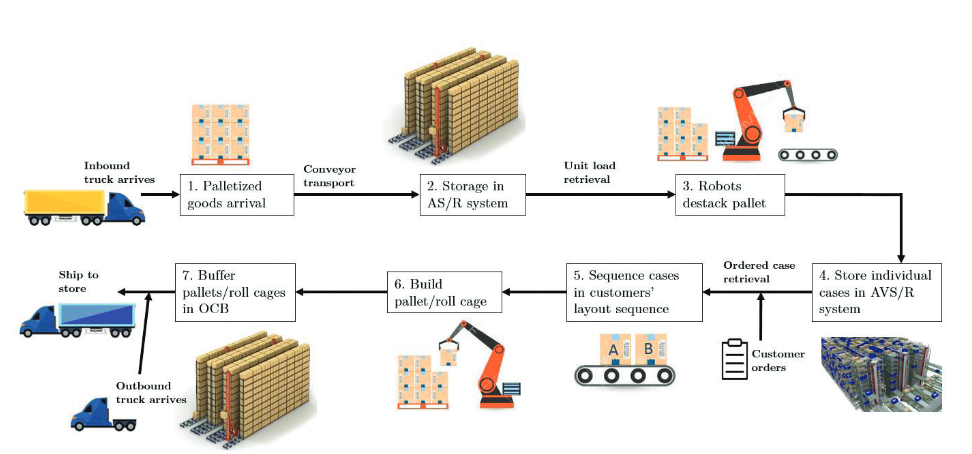
\includegraphics[width=0.8\textwidth]{../bachproef/img/warehousing_flow.png}
  \caption[Flow in a typical fully automated warehouse]{\label{fig:warehousing-flow}Standaard flow in een automatisch magazijn~\autocite{Koster2018}}
\end{figure}

\subsection{Handmatige systemen}
In deze soort beweegt de orderpicker zich naar de goederenlocaties, vaak met behulp van voertuigen zoals pickkarren of heftrucks. 
Deze systemen worden ook wel picker-to-product systemen genoemd, waarbij de medewerker fysiek de benodigde items verzamelt. 
Handmatige systemen zijn eenvoudig maar tijdrovend en vereisen veel arbeidskracht~\autocite{Berg1999}.

\subsection{Automatische systemen}
In deze systemen worden producten naar de orderpicker gebracht, vaak via ASRS-systemen (Automated Storage and Retrieval Systems). 
Dit zijn product-to-picker systemen waarbij de items automatisch worden verplaatst naar een vast pickpunt. 
Geautomatiseerde systemen kunnen de efficiëntie aanzienlijk verhogen door de reistijd van de orderpickers te verminderen 
en het picken te versnellen~\autocite{Berg1999}.
Het domein van dit onderzoek richt zich op het geautomatiseerde systeem. 

\subsection{Programmable Logic Controllers (PLC’s) in Warehousing}
Om een automatisch magazijn effectief aan te sturen, spelen Programmable Logic Controllers (PLC's) een cruciale rol.
PLC's zijn oorspronkelijk ontwikkeld om elektromechanische relais te digitaliseren in de industriële automatisering~\autocite{Bolton2015}. 
Door hun betrouwbaarheid, veelzijdigheid en robuustheid worden PLC’s breed toegepast in de industriële sector, waaronder in warehousing. 
In een magazijnomgeving monitoren en besturen PLC's tal van processen, zoals het transporteren van goederen, 
het positioneren van kranen en liften, en het uitvoeren van laad- en losactiviteiten.
Logistieke software wordt vaak gebruikt om bepaalde orders door te geven aan een PLC.

\subsection{Warehouse Control System (WCS) in Warehousing} 
In het magazijn is de typische logistieke software het Warehouse Control System (WCS). 
Het WCS biedt een geïntegreerde interface voor een breed scala aan apparatuur waaronder de PLC's. 
Het systeem kan de apparatuur in het magazijn beheren en aansturen~\autocite{Son2015}. 
Binnen het bedrijf is het WCS een onderdeel van het monolithische ERP-pakket, waarvan TVH de eigenaar is van de code, 
geschreven in OpenEdge Progress 4GL.
 
\section{OpenEdge Progress 4GL} 
Progress 4GL, ofwel "Fourth-Generation Language", is een programmeertaal ontwikkeld door Progress Software Corporation, 
die zich richt op bedrijfsapplicaties, vooral die met veel database-interacties. 
Het biedt een vereenvoudigde syntaxis, waarmee ontwikkelaars snel toepassingen kunnen bouwen voor zakelijke omgevingen.
Dankzij de optimalisatie voor databasebewerkingen is het geschikt voor toepassingen in sectoren als financiën en logistiek, 
waar real-time datatoegang essentieel is.

\section{Communicatie tussen PLC en WCS}
Een essentieel aspect van een geautomatiseerd magazijn is de soepele communicatie tussen de Programmable Logic Controllers (PLC’s) en 
het Warehouse Control System (WCS). 
Deze communicatie stelt het WCS in staat om gedetailleerde commando’s te sturen naar de PLC’s en om statusinformatie terug te ontvangen over de huidige staat van het magazijn en de apparatuur. 
Een stabiele en snelle datastroom tussen deze systemen is cruciaal voor een efficiënte werking en het minimaliseren van stilstand of fouten.

\subsection{Industriële protocollen voor communicatie} 
De communicatie tussen PLC’s en WCS kan worden gerealiseerd door middel van verschillende industriële protocollen, 
afhankelijk van de specificaties en vereisten van het magazijn en de gekozen hardware. 
Veelgebruikte protocollen zijn:

\subsubsection{Modbus}
Een relatief eenvoudig protocol dat oorspronkelijk ontwikkeld werd voor communicatie tussen PLC’s en sensoren of actuatoren. 
Het is een van de oudste protocollen en wordt nog steeds vaak gebruikt vanwege de eenvoud en lage kosten~\autocite{Joshi2024}. 

\subsubsection{Profinet}
Dit protocol biedt hoge snelheden en real-time communicatie 
en wordt vaak toegepast in grootschalige industriële automatiseringsprojecten, waaronder magazijnbeheer. 
Profinet is zeer geschikt voor situaties waarin hoge eisen worden gesteld aan nauwkeurigheid en stabiliteit.
Deze wordt gebruikt in het bedrijf om te communiceren tussen de PLC's.

\subsubsection{Ethernet/IP}
Dit protocol is gebaseerd op standaard TCP/IP en wordt veel gebruikt in de industrie vanwege de snelheid en flexibiliteit ~\autocite{Joshi2024}. 
Ethernet/IP ondersteunt real-time communicatie, wat essentieel is voor de snelle reactietijden die nodig zijn in een geautomatiseerd magazijn.
Dit protocol maakt gebruik van standaard Ethernet-hardware, zoals kabels, switches en routers. 
Dit vereenvoudigt de installatie en het onderhoud in industriële omgevingen en maakt het compatibel met bestaande IT-infrastructuur.
De PLC die deel uitmaakt van dit onderzoek, wisselt data uit van en naar het WCS via dit protocol.

\subsection{Data uitwisseling} 
Tijdens de samenwerking tussen PLC’s en het WCS worden er verschillende datastromen uitgewisseld via het Ethernet/IP netwerk.
Commando’s van WCS naar PLC: Het WCS stuurt instructies naar de PLC’s om specifieke handelingen uit te voeren, zoals het starten van een transportband of het positioneren van een kraan.
Statusupdates van PLC naar WCS: De PLC’s geven informatie terug aan het WCS over de huidige status van apparatuur. Bijvoorbeeld, of een transportband in werking is, 
de locatie van een item in het magazijn, en of er storingen of onderbrekingen zijn~\autocite{Laar2013}.

\subsection{Real-time monitoring en optimalisatie} 
Het WCS maakt gebruik van real-time data om de operaties in het magazijn optimaal te coördineren. 
Door continue monitoring kan het systeem bijvoorbeeld inspelen op piekperiodes door bijvoorbeeld geen bakken meer te laten uitsturen. 
Dit niveau van controle helpt magazijnen om de doorlooptijden te verkorten en de efficiëntie te maximaliseren.

\subsection{Voorbeeld: Integratie bij TVH} 
In het geval van TVH, waar het WCS onderdeel uitmaakt van een monolithisch ERP-systeem geschreven in OpenEdge Progress 4GL, 
vereist de communicatie tussen WCS en PLC’s een aangepaste interface. 
Dit ERP-systeem bevat een grote hoeveelheid bedrijfslogica en data over de voorraad, orderverwerking en logistiek.
Hierdoor heeft het ERP-systeem toegang tot alle informatie die nodig is om het magazijnproces aan te sturen. 
De interface met de PLC’s van Vanderlanden, zorgt ervoor dat het ERP-systeem commando’s kan versturen en statusinformatie kan ontvangen. 

\subsubsection{WCS communicatie} 
Op het ERP-systeem van TVH draaien acht verschillende batches die verantwoordelijk zijn voor de aansturing van de PLC. 
Elke batch-instantie communiceert met specifieke PLC-kanalen en bevat daarvoor specifieke logica.
Deze batches zijn verbonden via een specifieke poort met een Progress SonicMQ Adapter op de communicatie server.
Hiermee kunnen de batches de berichten consumeren en versturen van de SonicMQ server.

\subsubsection{Communicatie tussen PLC en WCS}
De PLC kan alleen maar een TCP/IP socket verbinding initiëren met een server.
Omdat SonicMQ als middleware hierdoor geen verbinding kan maken zijn er listeners gemaakt in Java door TVH.
Deze listeners fungeren als server en zijn specifiek opgesteld om een TCP/IP socket verbinding mogelijk te maken per PLC kanaal.
De Java listeners sturen de PLC-berichten vervolgens door naar SonicMQ of ontvangen berichten van SonicMQ, 
die ze via een socket naar de PLC doorsturen.
Aan de kant van het WCS zijn er meer mogelijkheden om verbinding te kunnen maken met een server.
 
\subsection{Uitdagingen en Toekomstige Ontwikkelingen} 
TODO:
\\
Er zijn enkele uitdagingen bij de integratie van PLC’s en WCS. 
Ten eerste zijn er eisen op het gebied van snelheid en betrouwbaarheid, aangezien zelfs kleine vertragingen in communicatie de doorstroming in het magazijn kunnen beïnvloeden. 
Daarnaast kunnen compatibiliteitsproblemen optreden, vooral wanneer er verouderde of verschillende generaties hardware en software binnen één systeem gebruikt worden.

In de toekomst kan de integratie tussen PLC’s en WCS verder verbeterd worden door de toepassing van nieuwe technologieën zoals Industrial Internet of Things (IIoT) en edge computing. 
Deze technologieën kunnen helpen om data nog sneller te verwerken en meer gedetailleerde inzichten te bieden in real-time, wat de flexibiliteit en efficiëntie van magazijnen kan verhogen.

Al met al vormt de communicatie tussen PLC’s en WCS een kritieke succesfactor voor een goed functionerend, geautomatiseerd magazijn, waar real-time aansturing en monitoring de sleutel zijn tot een snelle en betrouwbare logistieke operatie.
In dit onderzoek behouden we de scope op messaging systemen die communiceren via het Ethernet/IP netwerk.

\section{Communicatie methodes}
Dit hoofdstuk bevat informatie over de relevante communicatiemethoden en geeft inzicht in hun werking.
\\
\emph{Inter-Process Communication (IPC)} omvat alle vormen van communicatie tussen services, 
zowel binnen hetzelfde systeem als via een netwerk. 
Hieronder worden enkele methoden van \emph{Message Passing} toegelicht.

\subsection{Socket gebaseerd (TCP/UDP)}
Een socket-verbinding (TCP/IP) maakt gebruik van een endpoint gespecificeerd met een IP-adres en een poortnummer, 
waarmee twee autonome processen verbonden zijn, hetzij op dezelfde, hetzij op verschillende machines.
\\
\\
Streaming sockets (op basis van TCP) zijn nuttig voor betrouwbare, sequentiële berichtoverdracht.
Deze methode wordt gebruikt voor de connectie tussen de PLC en het WCS.
\\ 
\\
Datagram sockets (op basis van UDP) zijn geschikt zijn voor snelle, maar minder betrouwbare communicatie en wordt gebruikt voor bijvoorbeeld audio en video.
Beiden ondersteunen communicatie tussen verschillende netwerken en zijn veelgebruikt in messaging-applicaties~\autocite{Dinari2020}.

\subsection{Message queue gebaseerd}

\subsubsection{Publish-subscribe-model}
Het publish-subscribe-model is gebaseerd op topics waarop berichten worden gepubliceerd door de \emph{producer} 
en waar meerdere \emph{subscribers} (abonnees) zich kunnen op inschrijven~\autocite{Dinari2020}. 
\\
In dit model ontvangen \emph{subscribers} slechts een subset van de totale gepubliceerde berichten. 
Het proces van het selecteren en verwerken van de berichten wordt filtering genoemd. 
Er zijn twee vormen van filtering: op basis van onderwerp (topic) en op basis van inhoud (content).
\\
In een op \emph{topic} gebaseerd systeem worden berichten geplaatst in \emph{topics} wat logische kanalen zijn.
\emph{Subscribers} ontvangen berichten van de \emph{topics} waarop ze zich hebben geabonneerd.
Alle \emph{subscribers} ontvangen dezelfde berichten uit dezelfde \emph{topics}. 
Deze methode zorgt voor een \emph{one-to-many} vorm van communicatie~\autocite{Dinari2020}.
\\
Hierdoor ontvangen subscribers alleen de berichten uit de klassen die voor hen relevant zijn, zonder enige kennis van de publishers. 
Met het publish-subscribe-model specificeert de afzender nooit expliciet wie de ontvanger is en weet het zelfs niet of er al dan niet ontvangers zijn.

\begin{figure}[h!]
  \centering
  \includegraphics[width=.4\textwidth]{../voorstel/img/fig1-publish-subscribe.png}
  \caption{\label{fig:pub-sub}Publisher-Subscriber system~\autocite{Sharvari2019}.}
\end{figure}

\subsubsection{Point-to-Point-model}
Dit model wordt gebruikt door het huidige messaging systeem in het bedrijf.
Hier worden berichten door \emph{publishers} in specifieke wachtrijen geplaatst, genaamd queues waarna andere nodes, genaamd \emph{consumers} ze eruit halen. 
\\
Messaging queues hebben een asynchrone werking, zijn \emph{socket-based} en maken gebruik van \emph{message queuing}, 
waarbij het de \emph{point-to-point} methodiek gebruikt.
Hierbij plaatst de \emph{producer} berichten in een specifieke queue, waarna een \emph{consumer} de berichten uitleest in een sequentiële volgorde.
Met andere woorden, een bericht wordt slechts aan één \emph{consumer} bezorgt.
\\
Dit maakt het voor applicaties mogelijk om asynchroon te communiceren zonder te moeten wachten op een antwoord van de ontvanger.
Ze zijn geschikt voor gedistribueerde systemen waar processen onafhankelijk werken~\autocite{Dinari2020}.

\begin{figure}[h!]
  \centering
  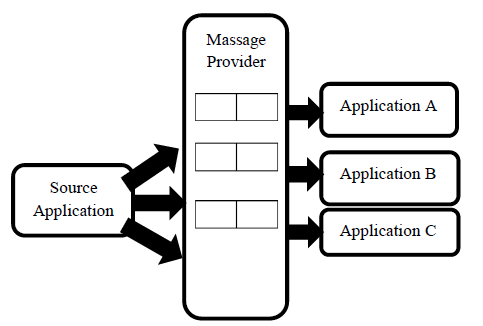
\includegraphics[width=.4\textwidth]{../bachproef/img/point-to-point-messaging.png}
  \caption{\label{fig:point-to-point}Point-to-point system~\autocite{Dinari2020}}
\end{figure}

\subsection{Niet relevante protocollen}
\subsubsection{RPC-methoden voor messaging}
In dit hoofdstuk worden de meest relevante \emph{Remote Procedure Call} (RPC) methoden besproken. 
Deze communicatiemethode is synchroon, wat betekent dat de verzendende partij moet wachten op een antwoord.
Hierdoor is deze manier van communiceren niet optimaal voor het domein van dit onderzoek, 
aangezien het niet de vereiste prestaties levert. 
Desondanks worden deze methoden besproken om inzicht te geven in hoe ze werken en om aan te tonen waarom ze niet geschikt zijn.

\subsubsection{XML en SOAP}
Deze methoden zijn relevant voor communicatie omdat ze methoden en objecten via XML over HTTP kunnen aanroepen,
wat communicatie mogelijk maakt tussen verschillende platformen en programmeertalen.
Zoals eerder besproken zijn deze synchroon waardoor de snelheid nadelig beïnvloed wordt.

\subsubsection{REST}
RESTful webservices gebruiken HTTP-verzoeken (zoals GET, POST) voor eenvoudige en efficiënte berichtuitwisseling en is heeft ook een synchrone werking. 
De berichten, meestal in JSON formaat, maakt dit geschikt voor communicatie tussen webapplicaties.

\subsection{Pipes}
\emph{Named pipes} hebben een synchrone werking en voorzien een bidirectionele 
communicatie tussen onafhankelijke processen.
Deze maakt het mogelijk om te kunnen functioneren tussen processen op hetzelfde systeem.
\\
\emph{Ordinary pipes} bieden beperkte eenzijdige communicatie en vereisen een parent-child relatie, 
wat ze minder geschikt maakt voor communicatie tussen onafhankelijke processen~\autocite{Dinari2020}.

\subsection{Shared memory}
Deze methode is niet relevant voor dit onderzoek omdat het gericht is op het delen van geheugenruimte 
tussen processen op hetzelfde systeem. 
Ze zijn nuttig voor het efficiënt delen van grote hoeveelheden data binnen hetzelfde systeem~\autocite{Dinari2020}.

\section{Synchroon vs. asynchroon}
Services communiceren zowel \emph{synchroon} als \emph{asynchroon} en spelen deze benaderingen een cruciale rol, 
elk met hun eigen voor- en nadelen. \emph{Synchrone microservices} werken volgens een direct 
afhankelijkheidsmodel, omdat services met elkaar communiceren in een vraag-antwoordpatroon. 
Deze synchrone communicatie kan leiden tot ingewikkelde onderlinge afhankelijkheden, vertragingen en complexiteiten bij het debuggen 
van de logica. Bovendien wordt het schalen van synchrone services uitdagend, 
aangezien de schaalbaarheid van één service sterk afhankelijk is van andere services die het gebruikt \autocite{Bellemare2020}. 
Deze manier van communicatie kan niet voldoen aan de niet-functionele eisen van het automatisch magazijn binnen TVH.
\newline

Daartegenover heeft \emph{asynchrone} communicatie een reeks voordelen. Ze bieden grotere schaalbaarheid, technologische 
flexibiliteit en aanpassingsvermogen aan veranderende zakelijke vereisten. 
In plaats van de synchrone manier van communicatie is de \emph{asynchrone} gemakkelijker te herstructureren en te onderhouden. 
Ze vergemakkelijken \emph{continuous delivery} door hun onafhankelijkheid omdat de communicatie 
met een \emph{messaging systeem} opgevangen wordt. 
Hun verminderde afhankelijkheden en geïsoleerde karakter maken het testen relatief eenvoudiger en robuuster.
Het enige grote nadeel in asynchrone communicatie is \emph{error handling}, 
omdat dit niet opgevangen kan worden door de verzendende partij.
\newline

\begin{figure}[h!]
  \centering
  \includegraphics[width=.5\textwidth]{../voorstel/img/synchronous_vs_async_calls.png}
  \caption{\label{fig:sync-vs-async}Synchronous versus asynchronous communication \autocite[figure 14 -- 13]{MarkRichards2021}.}
\end{figure}

In praktische termen is het vinden van de juiste balans tussen synchrone en \emph{asynchrone microservices} cruciaal, 
afhankelijk van de specifieke behoeften van een organisatie en de aard van haar bedrijfsprocessen. 
Een hybride aanpak waarin beide architecturen naast elkaar bestaan en elkaar aanvullen blijkt vaak de meest effectieve strategie te zijn. 
Deze aanpak stelt organisaties in staat om de sterke punten van zowel synchrone als asynchrone modellen te benutten, 
waardoor flexibiliteit, schaalbaarheid en onderhoudsgemak worden gegarandeerd in complexe \newline IT-landschappen.
In deze paper ligt de focus op \emph{asynchrone communicatie} voor het gebruik van \emph{messaging systemen}.
\newline

\section{Cloud vs. On-premise}
Dit hoofdstuk vergelijkt cloud- en on-premise-oplossingen, waarbij de verschillen, voordelen en uitdagingen van beide opties worden belicht. 
Cloud-oplossingen draaien op externe servers die via het internet toegankelijk zijn, 
terwijl on-premise-oplossingen lokaal binnen de eigen infrastructuur worden beheerd en onderhouden.
De snelheid over het netwerk kan onderzocht en getest worden voor beide toepassingen en is relevant voor het aanbevelingsrapport.

\subsubsection{Cloud}
In het cloud model worden hardware, software en applicaties extern beheerd door een serviceprovider, wat zorgt voor meer flexibiliteit. 
Organisaties kunnen functies toevoegen of verwijderen op basis van veranderende behoeften.
\\
De cloud is doorgaans kostenefficiënter, aangezien organisaties alleen betalen voor de gebruikte resources, 
in plaats van grote initiële investeringen in hardware en software~\autocite{Golec2021}.
Beveiliging blijft een zorg, maar de cloud biedt uitgebreide beveiligingsmaatregelen en beleidsregels, inclusief speciale cloud omgevingen voor gevoelige data. 
De Europese Commissie heeft Codes of Conduct ontwikkeld om de data te beschermen.
Onderhoud wordt volledig door de cloud provider verzorgd, inclusief automatische updates en upgrades, zonder extra kosten behalve voor de gebruikte hardware.
Cloud oplossingen bieden meer schaalbaarheid en flexibiliteit. 
Infrastructuur kan snel worden aangepast aan veranderende behoeften, wat sneller en eenvoudiger is dan bij on-premises modellen.

\subsubsection{On-Premise}
Bij on-premises oplossingen beheert de organisatie zelf de hardware, software en applicaties op locatie in het eigen datacenter, wat meer controle en verantwoordelijkheid vereist.
De huidige setup voor de communicatie tussen PLC en WMS is on-premise opgesteld.
On-premises systemen brengen hogere initiële kosten met zich mee voor hardware en software, 
en organisaties zijn verantwoordelijk voor het onderhoud van servers, data-back-ups en disaster recovery~\autocite{Golec2021}.
De beveiliging is volledig in eigen handen, wat voor sommige organisaties een voordeel kan zijn, maar ook extra zorg en middelen vereist.
Organisaties moeten zelf zorgen voor onderhoud en updates van de infrastructuur, wat tijdrovend kan zijn en extra kosten met zich meebrengt.
Schaalbaarheid is beperkter; het aanpassen van de infrastructuur of het uitbreiden van servers is een tijdrovend proces in vergelijking met de cloud.
Een groot voordeel hier is de volledige controle en dat er geen afhankelijkheden zijn van derden.

\section{Messaging protocollen}

\subsection{AMQP (Advanced Message Queuing Protocol)} 

\subsection{STOMP (Streaming Text Orientated Messaging Protocol)}

\subsection{MQTT (Message Queue Telemetry Transport)}

\section{Messaging-Technologieën}


\section{Wat is een EoL systeem}

\subsection{Wat zijn de gevaren van EoL systemen}

\subsection{Welke manieren zijn er om EoL weg te werken}










%%=============================================================================
%% Methodologie
%%=============================================================================

\chapter{\IfLanguageName{dutch}{Methodologie}{Methodology}}%
\label{ch:methodologie}

%% TODO: In dit hoofstuk geef je een korte toelichting over hoe je te werk bent
%% gegaan. Verdeel je onderzoek in grote fasen, en licht in elke fase toe wat
%% de doelstelling was, welke deliverables daar uit gekomen zijn, en welke
%% onderzoeksmethoden je daarbij toegepast hebt. Verantwoord waarom je
%% op deze manier te werk gegaan bent.
%% 
%% Voorbeelden van zulke fasen zijn: literatuurstudie, opstellen van een
%% requirements-analyse, opstellen long-list (bij vergelijkende studie),
%% selectie van geschikte tools (bij vergelijkende studie, "short-list"),
%% opzetten testopstelling/PoC, uitvoeren testen en verzamelen
%% van resultaten, analyse van resultaten, ...
%%
%% !!!!! LET OP !!!!!
%%
%% Het is uitdrukkelijk NIET de bedoeling dat je het grootste deel van de corpus
%% van je bachelorproef in dit hoofstuk verwerkt! Dit hoofdstuk is eerder een
%% kort overzicht van je plan van aanpak.
%%
%% Maak voor elke fase (behalve het literatuuronderzoek) een NIEUW HOOFDSTUK aan
%% en geef het een gepaste titel.

Volgende hoofdstukken verlopen in sequentiële volgorde om dit onderzoek in de juiste richting te sturen.
De literatuurstudie geeft een basis om verdere vakterminologie en de werking van technologieën te kunnen begrijpen.
\\
De opzet van het huidige systeem wordt besproken om de requirements te kunnen begrijpen.
Het bekomen van een shortlist wordt toegelicht waarbij voor elke technologie de voor- en nadelen wordt beschreven.

\section{Phase 1: Literatuurstudie}
Voor dit onderzoek werden de vaktermen opgesomd en onderverdeeld in groepen met behulp van een mindmap.
Vervolgens werd er gebruik gemaakt van het internet om wetenschappelijke artikelen op te zoeken om de nodige informatie uit te filteren.
\\
Het doel van de literatuurstudie is om een basis van bestaande kennis te verkrijgen door de belangrijkste concepten toe te lichten die van toepassing zijn op dit onderzoek. 
Dit houdt in, het begrijpen van warehousing, WCS (Warehouse Control Systems), PLC (Programmable Logic Controllers), en de communicatieprotocollen die tussen deze systemen gebruikt worden.
\\
Hierdoor krijg je een overzicht van relevante theorieën, definities, en eerdere studies die inzicht geven in de werking en de gebruikte technologieën.
Er werd voornamelijk gebruik gemaakt van wetenschappelijke artikelen, boeken en technische documenten.
\\
De literatuurstudie vormt de basis van het onderzoek en is cruciaal voor het begrijpen van de huidige stand van zaken.
Hierdoor kan de kennis en vereisten meegenomen worden doorheen de methodologie.

\section{Phase 2: Long List}
Dit hoofdstuk vertrekt vanuit een lijst met message brokers die beschikbaar zijn op de markt.
Deze worden later gefilterd door bepaalde criteria toe te passen, waarna de overgebleven kandidaten getest kunnen worden.
Op deze manier worden alle mogelijke opties geargumenteerd.

\subsection{Beschikbare messaging software}
Deze lijst bevat relevante message brokers als startpunt die beschikbaar zijn op de markt.
Bronnen werden geraadpleegd via zoekmachines, forums en blogs.

\begin{table}[!h]
\footnotesize
\centering
\begin{tabular}{|l|c|c|c|c|c|}
\hline
Message Broker & JMS & Linux & Protocollen & Kostenmodel & On premise \\
\hline
Apache Kafka & Ja & Ja & Kafka, MQTT, REST & Open-source & Ja \\
\hline
RabbitMQ & Ja & Ja & AMQP, MQTT, STOMP & Open-source & Ja \\
\hline
ActiveMQ & Ja & Ja & AMQP, MQTT, STOMP, OpenWire & Open-source & Ja \\ 
\hline
Artemis & Ja & Ja & AMQP, MQTT, STOMP & Open-source & Ja \\
\hline
MQTT.js & Ja & Ja & MQTT & Open-source & Ja \\
\hline
IBM MQ & Ja & Ja & MQ, MQTT & Abonnement & Ja \\
\hline
Redis & Ja & Ja & Stream, Pub/Sub & Open-source & Ja \\
\hline
NSQ & Ja & Ja & Stream, Pub/Sub & Open-source & Ja \\
\hline
Apache Pulsar & Ja & Ja & Stream, Pub/Sub & Open-source & Ja \\
\hline
NATS & Ja & Ja & NATS & Open-source & Ja \\
\hline
ZeroMQ & Ja & Ja & ØMQ (Socket) & Open-source & Ja \\ 
\hline
Amazon SQS & Nee & Nee & AWS protocol & Pay-per-use & Nee \\
\hline
Google Cloud Pub/Sub & Nee & Nee & Cloud Pub/Sub & Pay-per-use & Nee \\
\hline
Azure Service Bus & Nee & Nee & AMQP, MQTT, HTTP & Pay-per-use & Nee \\
\hline
Solace PubSub+ & Ja & Nee & AMQP & Pay-per-use & Nee \\
\hline
\end{tabular}
\caption{\label{tab:message_brokers}Longlist message brokers}
\end{table}

\section{Phase 3: Requirements analyse van huidige setup}
Dit hoofdstuk gaat dieper in op de huidige setup en werking tussen het WCS, messaging software en de PLC's.
Documenten van het bedrijf en interviews met vakexperts vormen de basis voor dit overzicht.
\\
Het doel is om na het lezen van dit hoofdstuk inzicht te krijgen in de requirements van het huidige systeem, 
zodat deze kunnen dienen als basis voor de keuze van een surrogaat voor het huidige messaging systeem.

\subsection{PLC gebruik binnen TVH}
Er zijn 7 verschillende PLC's in TVH Waregem die instaan voor verschillende zones van de conveyor.
Deze werden aangeleverd door Vanderlanden in het jaar 2013 en worden beheerd door het automatisatieteam.
De communicatie tussen een PLC en het WCS is gebaseerd op het TCP/IP-protocol en is verbonden via het intern netwerk.
Er is een tussenlaag tussen de PLC en het netwerk, RFC1006 van het merk Siemens waarin configuratie kan worden gedaan door het automatisatie team.
Dit stelt de collega's in staat om bepaalde logica te implementeren of netwerk aanpassingen door te voeren.
De snelheid van communicatie is essentieel, daarom moet het netwerk snel genoeg zijn zodat berichten aan een snel tempo verstuurd kunnen worden.
\\\\
De PLC's maken gebruik van een TCP/IP-socketverbinding en functioneren als client ten opzichte van het WCS, dat de rol van server vervult. 
Dit betekent dat de PLC de verbinding initieert en persisteert met de server die verantwoordelijk is voor de communicatie.
Een PLC is verantwoordelijk voor een specifieke zone van de conveyor en is opgebouwd uit drie kanalen die elk via een toegewezen poortnummer met de server communiceren. 
Meerdere kanalen zijn nodig om de communicatiesnelheid te bevorderen en omdat elk kanaal zijn eigen type informatie verwerkt.

\begin{table}[!h]
  \centering
  \begin{tabular}{lcr}
    \toprule
    \textbf{Kanaal} & \textbf{Beschrijving} & \textbf{Type}                        \\
    \midrule
    1                & Route informatie over transportbak          & Snel           \\
    2                & Informatie van PLC                          & Niet kritisch  \\
    3                & Overige informatie over transportbak        & Snel           \\
    \bottomrule
  \end{tabular}
  \caption[Channel assignment]{\label{tab:channel-assignment}Beschrijving van kanalen}
\end{table}

\subsubsection{PLC berichten}
Berichten bestaan uit een frame opgedeeld in velden en hebben een specifieke lengte.
De inhoud van een bericht is gebaseerd op het hexadecimale stelsel en wordt in detail toegelicht in de onderstaande tabel.
\begin{table}[h!]
\centering 
\begin{tabular}{|c|c|c|c|}
  \hline
  \textbf{Veld} & \textbf{Inhoud} & \textbf{Data type} & \textbf{Lengte} \\
  % \hline
  % Dummy & Enkel PLC naar WCS
  \hline 
  Header & <STX> & Binair & 1 byte \\
  \hline 
  Lengte in bytes & 001D(HEX) & Binair & 2 bytes \\
  \hline 
  Seq. nummer &  [0-9] & ASCII & 1 byte  \\
  \hline 
  Inhoud & <...> & Binair & 27 bytes \\
  \hline 
  Terminator & <ETX> & Binair & 1 byte \\
  \hline
\end{tabular}
\caption[Message content]{\label{tab:message-content}Inhoud bericht}
\end{table}

Bepaalde controles worden uitgevoerd om de validiteit van een bericht af te toetsen. 
\\\\
Er worden ongeveer 80 berichten per minuut verstuurd per PLC, per kanaal.
Het totale aantal verstuurde berichten per minuut komt uit op ongeveer 1680/min.

Voorbeeld van een bericht dat van PLC naar WCS wordt verstuurd: 
\begin{listing}[h!]
\begin{minted}{python}
  02 00 1d 20 30 36 20 20 00 00 20 20 30 37 20 20 30 20 20 20 20 20 20 20 20 20 20 20 20 20 20 03
\end{minted}
\caption[Voorbeeld PLC bericht]{\label{listing:message_example}Voorbeeld van een PLC bericht}
\end{listing}

\subsection{Java listeners}
De PLC kan uitsluitend maar een TCP/IP-socket verbinding initiëren met een server.
Omdat SonicMQ als middleware hierdoor geen verbinding kan maken zijn er Java-listeners gemaakt door TVH.
Deze listeners fungeren als server en zijn specifiek opgesteld om een TCP/IP-socket verbinding mogelijk te maken per PLC kanaal.
De Java-listeners sturen de PLC-berichten vervolgens door naar SonicMQ of ontvangen berichten van SonicMQ, 
die ze via een socket naar de PLC doorsturen.
Aan de kant van het WCS zijn er meer mogelijkheden om verbinding te kunnen maken met een server.
SonicMQ biedt geen support meer en is niet populair waardoor er ook geen community is.
Dit kan leiden tot extra kosten of langdurige problemen.

\subsection{WCS communicatie} 
Op het ERP-systeem van TVH draaien acht verschillende batches die verantwoordelijk zijn voor de aansturing van de PLC. 
Elke batch-instantie communiceert met specifieke PLC-kanalen en bevat daarvoor specifieke logica, geschreven in OpenEdge Progress 4GL.
Deze batches zijn verbonden via een specifieke poort met een \textbf{Progress JMS Adapter} op de communicatieserver omdat ze de ``Broker connect'' methode gebruiken.
Hiermee kunnen de batches de berichten consumeren en versturen van de SonicMQ server.
Daarnaast is het ook mogelijk om de Client connect methode te gebruiken, wat gemakkelijker is qua integratie.

\subsubsection{Progress OpenEdge JMS Adapter}
De adapter stelt OpenEdge-applicaties in staat om berichten te verzenden en te ontvangen van JMS (Java Messaging System)
messagebrokers zoals Apache ActiveMQ. 
Dit betekent dat OpenEdge-applicaties kunnen integreren met andere systemen die JMS ondersteunen, 
zonder dat er directe afhankelijkheden nodig zijn.
Hierdoor is de keuze van message brokers gelimiteerd tot brokers die \textbf{JMS ondersteunen}.

\subsubsection{Integratie met Verschillende Enterprise Systemen}
Met de JMS Adapter kunnen OpenEdge-applicaties communiceren met andere systemen zoals ERP en CRM-systemen, 
wat nuttig is in bedrijfsprocessen waarbij gegevens moeten worden gedeeld tussen verschillende systemen.

\subsubsection{Configuratie en Beheer}
De Progress OpenEdge JMS Adapter biedt configuratiemogelijkheden waarmee beheerders de communicatie kunnen aanpassen 
aan de vereisten van hun omgeving, zoals het instellen van queue-namen, topics, verbindingsparameters, en het beheren van uitzonderingen.

\subsubsection{WCS berichten} 
Berichten komen binnen van de PLC via de communicatie server. Ieder bericht wordt getransformeerd naar variabelen die dan verder gebruikt worden in de code.
Deze berichten bevatten informatie over transportbakken en zijn nodig om deze te kunnen traceren via de ERP.
Specifieke logica is nodig om bakken tot hun bestemming te krijgen, of om fout afhandeling te voorzien.
\\\\
Volgende voorbeelden doen zich voor:
\begin{enumerate}
\item Routeren naar een hospitaal punt door: 
\begin{enumerate}
  \item Gewichtsfout
  \item Hoogtefout
  \item Onbekende bestemming
\end{enumerate}
\item Bestemming wordt gevraagd door de PLC
\item Bestemming wordt doorgegeven aan de PLC 
\item Specifieke logica moet uitgevoerd worden bij het passeren van een bepaald punt
\item \dots
\end{enumerate}

\subsection{Monitoring}
Het bestaande systeem wordt visueel gemonitord met behulp van Grafana en Elastic. 
Voor het ophalen van de logging wordt gebruik gemaakt van Prometheus.
Hierdoor kunnen systeemfouten snel opgemerkt worden en berichten verstuurd worden als bepaalde waardes overschreden worden.
\newpage

\subsection{Samenvatting requirements messaging systeem}
De belangrijkste requirements voor de huidige setup zijn als volgt:

\subsubsection{Integratie met het WCS systeem}
Het messaging systeem moet kunnen integreren met het huidige WCS-systeem dat gebruik maakt van Progress 4GL versie 11.7. 
Hiervoor moet de broker het \textbf{JMS protocol ondersteunen} en geïnstalleerd kunnen worden op een \textbf{Linux platform}.
Daarnaast moet de middleware ook gebruikt kunnen worden door \textbf{monitoring software}.

\subsubsection{Performantie}
Om de real-time eisen van het WCS en de PLC’s te ondersteunen, moet het messaging systeem \textbf{hoge performantie} bieden. 
Dit betekent dat berichten zonder merkbare vertraging moeten worden verstuurd en ontvangen, 
zodat de snelheid van de conveyor niet wordt beperkt door de communicatiesnelheid.
Om vertraging te voorkomen moet de verwerking van de berichten \textbf{asynchroon} gebeuren.

\subsubsection{Betrouwbare Berichtenoverdracht}
Het systeem moet in staat zijn berichten \textbf{consistent en zonder verlies} over te brengen. 
Dit is essentieel om de traceerbaarheid van transportbakken te garanderen en fouten in de logistieke processen te voorkomen.
Hiervoor moet de broker het \textbf{AMQP-protocol} ondersteunen.

\subsubsection{Support en Community}
Het is belangrijk dat de gekozen message broker support biedt en dat er een grote community aanwezig is 
waarbij je terecht kunt voor advies, probleemoplossing en best practices.
Daarnaast is het ook belangrijk dat er commerciële support beschikbaar is om SLA's (Service Level Agreement's) te kunnen afdwingen.

\subsubsection{Kosten}
Support gaat vaak samen met kosten en is ook belangrijk om mee te nemen in de keuze van een messaging systeem.
Sommige systemen hangen vast aan een kostenmodel, andere zijn \textbf{open-source} en zijn kosteloos.
\newpage
\subsubsection{MoSCoW prioriteiten}

\textbf{Must have:}
\begin{itemize}
\item Hoge performantie 
\item Asynchroon verzenden van gegevens  
\item JMS ondersteuning
\item Installatie mogelijk op Linux OS 
\item AMQP-protocol ondersteunen 
\item Monitoring mogelijkheden
\item Moet lokaal kunnen geïnstalleerd worden
\item Commerciële support
\end{itemize}

\textbf{Should have:}
\begin{itemize}
  \item Kostenmodel: open source 
  \item Uitgebreide documentatie
  \item Gemakkelijk op te schalen: om niet beperkt te worden in groei
  \item Gebruiksvriendlijkheid
\end{itemize}

\textbf{Could have}:
\begin{itemize}
  \item Actieve Community en support
  \item UI console via web pagina
  \item Integratie met huidig systeem
  \item Filtering op properties
\end{itemize}

\newpage
\section{Phase 5: ShortList}
In deze sectie worden de message brokers uit de longlist opgelijst en stapsgewijs gefilterd op basis van het MoSCoW principe.
Het doel is om een top 3 te bekomen waarbij uitvoerige testen kunnen uitgevoerd worden.

\subsection{Must have}
In deze sectie wordt de longlist van beschikbare messaging brokers gefilterd op basis van de gestelde must-have criteria. 
Messaging brokers die niet voldoen aan een van deze criteria worden verworpen, omdat de must-have eisen de hoogste prioriteit hebben.
\\\\
Voor elke technologie wordt een onderbouwde argumentatie gegeven op basis van de must-have criteria om de gemaakte keuzes inzichtelijk te maken. 
Het aspect van hoge prestaties, dat eveneens onderdeel is van de must-have criteria, wordt geëvalueerd tijdens de testen.
\\\\
Producten die voldoen aan de ``must-have'' criteria worden als kandidaat gemarkeerd en meegenomen naar de volgende stap, waarin ``should-have'' criteria worden toegepast.
 
\subsubsection{Apache Kafka}
\begin{itemize}
    \item \textbf{Hoge performantie:} Kafka biedt een uitstekende prestatie, met name bij het verwerken van grote hoeveelheden gegevens in real-time via events streaming ~\autocite{Ueberfuhr2024}.
    \item \textbf{Asynchroon verzenden van gegevens:} Ondersteunt volledig asynchrone gegevensverwerking en data-uitwisseling via streams.
    \item \textbf{JMS ondersteuning:} Beschikt niet over native JMS-ondersteuning, maar kan indirect worden geïntegreerd met JMS via extra adapters.
    \item \textbf{Installatie mogelijk op Linux OS:} Kafka kan eenvoudig worden geïnstalleerd en uitgevoerd op Linux-systemen.
    \item \textbf{AMQP protocol ondersteunen:} Ondersteunt geen direct AMQP-protocol, wat een belangrijke beperking vormt tegenover huidige setup.
    \item \textbf{Monitoring mogelijkheden:} Kafka biedt uitgebreide monitoringopties, inclusief integratie met tools zoals Prometheus en Grafana.
    \item \textbf{Moet lokaal kunnen geïnstalleerd worden:} Kan lokaal worden geïnstalleerd en beheerd, wat flexibiliteit biedt voor implementaties.
    \item \textbf{Commerciële support:} Beschikt over een grote en actieve community. Daarnaast bieden diverse bedrijven, zoals Confluent, betaalde ondersteuning aan.
    \item \textbf{Voldoet niet volledig aan de vereisten:} Het ontbreken van AMQP-ondersteuning en de incompatibiliteit met de huidige Progress OpenEdge 11.7-omgeving maken het niet geschikt voor de huidige setup.  
    Ondanks Kafka op dit moment niet kan worden gebruikt, blijft het een technologie die in de toekomst als kandidaat kan worden overwogen, 
    bijvoorbeeld bij een upgrade naar Progress OpenEdge 12.8 waar een Kafka-adapter beschikbaar is ~\autocite{Progress2024}.
\end{itemize}

 
\subsubsection{RabbitMQ}
\begin{itemize}
    \item \textbf{Hoge performantie:} RabbitMQ biedt uitstekende prestaties en is in staat grote hoeveelheden berichten snel en efficiënt te verwerken ~\autocite{baeldung2024}.
    \item \textbf{Asynchroon verzenden van gegevens:} Ondersteunt volledig asynchrone gegevensuitwisseling.
    \item \textbf{JMS ondersteuning:} Beschikt over JMS-ondersteuning, wat het geschikt maakt voor integratie in onze omgeving.
    \item \textbf{Installatie mogelijk op Linux OS:} Kan eenvoudig worden geïnstalleerd op diverse Linux-distributies.
    \item \textbf{AMQP protocol ondersteunen:} Ondersteunt AMQP, wat bijdraagt aan de veelzijdigheid en flexibiliteit van de broker.
    \item \textbf{Monitoring mogelijkheden:} RabbitMQ biedt uitgebreide monitoringmogelijkheden via tools zoals RabbitMQ Management Plugin, evenals integraties met externe monitoringoplossingen.
    \item \textbf{Moet lokaal kunnen geïnstalleerd worden:} Ondersteunt lokale installatie, wat belangrijk is voor onze setup.
    \item \textbf{Commerciële support:} Beschikt over een grote en actieve community. Daarnaast is professionele ondersteuning beschikbaar via onder andere Pivotal en andere aanbieders.
    \item \textbf{Voldoet aan de vereisten:} Met ondersteuning voor AMQP en JMS voldoet RabbitMQ aan de gestelde eisen en is het geschikt voor opname in de shortlist. 
    Daarnaast wordt de broker actief ontwikkeld, beschikt het over uitgebreide documentatie en biedt het mogelijkheden voor professionele ondersteuning.
\end{itemize}
  
\subsubsection{ActiveMQ Classic}
\begin{itemize}
    \item \textbf{Hoge performantie:} ActiveMQ Classic biedt solide prestaties en is geschikt voor een breed scala aan messaging-toepassingen ~\autocite{Reock2020}.
    \item \textbf{Asynchroon verzenden van gegevens:} Ondersteunt volledig asynchrone gegevensverwerking via verschillende protocollen.
    \item \textbf{JMS ondersteuning:} Native ondersteuning voor JMS, wat het ideaal maakt voor Java-gebaseerde toepassingen.
    \item \textbf{Installatie mogelijk op Linux OS:} Kan eenvoudig worden geïnstalleerd op moderne Linux-systemen en is ook geschikt voor cloudomgevingen.
    \item \textbf{AMQP protocol ondersteunen:} Ondersteunt AMQP, evenals andere protocollen zoals OpenWire, STOMP, en MQTT, wat het veelzijdig maakt.
    \item \textbf{Monitoring mogelijkheden:} Beschikt over monitoringopties via JMX, evenals integratiemogelijkheden met externe tools zoals Prometheus en Grafana.
    \item \textbf{Moet lokaal kunnen geïnstalleerd worden:} Kan lokaal worden geïnstalleerd, wat past binnen de eisen van de huidige infrastructuur.
    \item \textbf{Commerciële support:} Actieve communityondersteuning is beschikbaar, evenals commerciële ondersteuning via aanbieders zoals Red Hat en andere partijen.
    \item \textbf{Voldoet aan de vereisten:} ActiveMQ Classic is een bewezen, JMS-gebaseerde message broker die veelzijdige protocolondersteuning biedt en gratis beschikbaar is zonder licentiekosten. 
    Hoewel het een stabiele en betrouwbare oplossing is, verschuift de focus van de community langzaam naar ActiveMQ Artemis. 
    Dit kan betekenen dat toekomstige innovaties minder frequent zijn. Desondanks blijft ActiveMQ Classic een sterke keuze voor organisaties die een robuuste, kostenbesparende message broker zoeken.
\end{itemize}
 
\subsubsection{ActiveMQ Artemis}
\begin{itemize}
    \item \textbf{Hoge performantie:} ActiveMQ Artemis biedt hoge prestaties dankzij de geoptimaliseerde interne architectuur ~\autocite{JustinReock2023}.
    \item \textbf{Asynchroon verzenden van gegevens:} Ondersteunt volledig asynchrone berichtenverwerking, zelfs bij hoge doorvoersnelheden.
    \item \textbf{JMS ondersteuning:} Native ondersteuning voor JMS, waardoor het ideaal is voor Java-gebaseerde toepassingen.
    \item \textbf{Installatie mogelijk op Linux OS:} Kan eenvoudig worden geïnstalleerd op Linux-systemen en is geschikt voor moderne infrastructuren.
    \item \textbf{AMQP protocol ondersteunen:} Ondersteunt AMQP, evenals andere protocollen zoals OpenWire, MQTT en STOMP, wat de veelzijdigheid vergroot.
    \item \textbf{Monitoring mogelijkheden:} Beschikt over uitgebreide monitoringopties, inclusief JMX en integraties met tools zoals Prometheus en Grafana.
    \item \textbf{Moet lokaal kunnen geïnstalleerd worden:} Kan lokaal worden geïnstalleerd, wat flexibiliteit biedt voor on-premise implementaties.
    \item \textbf{Commerciële support:} Actieve communityondersteuning is beschikbaar, naast commerciële ondersteuning via bedrijven zoals Red Hat en andere aanbieders.
    \item \textbf{Voldoet aan de vereisten:}
    ActiveMQ Artemis is een moderne, open source JMS-gebaseerde message broker met een geavanceerde interne architectuur die uitstekende prestaties biedt ~\autocite{JustinReock2023}.
    Alle aspecten van dit systeem voldoen aan de criteria waardoor deze in de shortlist kan opgenomen worden.
\end{itemize}
 
 
\subsubsection{MQTT.js}
\begin{itemize}
    \item \textbf{Hoge performantie:} MQTT.js biedt uitstekende prestaties voor het implementeren van het MQTT-protocol ~\autocite{Yu2024}.
    \item \textbf{Asynchroon verzenden van gegevens:} Ondersteunt volledig asynchrone berichtenverwerking, wat zorgt voor lage latency en hoge doorvoersnelheid.
    \item \textbf{JMS ondersteuning:} MQTT.js biedt geen native ondersteuning voor JMS.
    \item \textbf{Installatie mogelijk op Linux OS:} MQTT.js is een bibliotheek dat gebruikt wordt bij de implementatie van browsers.
    \item \textbf{AMQP protocol ondersteunen:} Ondersteunt geen AMQP-protocol, maar is volledig geoptimaliseerd voor het MQTT-protocol.
    \item \textbf{Monitoring mogelijkheden:} Voor monitoring kan MQTT.js worden gecombineerd met andere tools, zoals MQTT-servers met ingebouwde monitoring of externe monitoringoplossingen.
    \item \textbf{Moet lokaal kunnen geïnstalleerd worden:} Kan lokaal geïnstalleerd worden in een Node.js-omgeving of geïntegreerd in browserapplicaties.
    \item \textbf{Commerciële support:} Als open source library heeft MQTT.js geen officiële commerciële ondersteuning, maar is er een grote actieve community die ondersteuning biedt via forums en GitHub.
    \item \textbf{Voldoet niet aan de vereisten:}  
    MQTT.js is geen geschikte kandidaat voor onze vereisten omdat het alleen het MQTT-protocol ondersteunt en geen ondersteuning biedt voor andere protocollen zoals AMQP of JMS, wat essentieel is voor onze toepassingen. 
    Daarnaast biedt het geen commerciële ondersteuning en heeft het beperkte monitoringmogelijkheden in vergelijking met andere brokers. 
\end{itemize}
 

\subsubsection{IBM MQ}
\begin{itemize}
    \item \textbf{Hoge performantie:} IBM MQ biedt uitstekende prestaties en is ontworpen voor enterprise-grade toepassingen met hoge beschikbaarheid en betrouwbaarheid ~\autocite{IBM2024}.
    \item \textbf{Asynchroon verzenden van gegevens:} Ondersteunt volledig asynchrone berichtenverwerking met garantie voor berichtlevering.
    \item \textbf{JMS ondersteuning:} Biedt volledige ondersteuning voor JMS, wat het ideaal maakt voor integratie met Java-gebaseerde toepassingen.
    \item \textbf{Installatie mogelijk op Linux OS:} IBM MQ kan draaien op Linux OS-omgevingen.
    \item \textbf{AMQP protocol ondersteunen:} Ondersteunt het AMQP-protocol.
    \item \textbf{Monitoring mogelijkheden:} Biedt uitgebreide monitoring- en beheeropties, inclusief integratie met externe tools voor gedetailleerde prestatieanalyse.
    \item \textbf{Moet lokaal kunnen geïnstalleerd worden:} Kan lokaal geïnstalleerd worden.
    \item \textbf{Commerciële support:} IBM MQ biedt commerciële ondersteuning via IBM zelf, met een gesloten community en uitgebreide documentatie.
    \item \textbf{Voldoet aan de vereisten:} IBM MQ is een robuuste JMS-gebaseerde message broker die veelzijdige protocolondersteuning biedt, waaronder AMQP. 
    Het biedt enterprise-grade functionaliteit, met garanties voor berichtlevering, beveiliging, en transactiebeheer. 
    De broker biedt uitgebreide functionaliteiten die het ideaal maken voor veeleisende toepassingen maar kan overkill zijn voor het huidige WCS systeem.
\end{itemize}
 

\subsubsection{Redis}
\begin{itemize}
    \item \textbf{Hoge performantie:} Redis is een in-memory data platform dat uitzonderlijke snelheid biedt voor berichtenverwerking ~\autocite{Saxena2024}.
    \item \textbf{Asynchroon verzenden van gegevens:} Ondersteunt asynchrone berichtenverwerking via pub/sub-mechanismen en streams.
    \item \textbf{JMS ondersteuning:} Redis ondersteunt JMS alleen via verschillende client bibliotheken, waardoor het minder direct compatibel is met systemen die native JMS vereisen.
    \item \textbf{Installatie mogelijk op Linux OS:} Redis is volledig compatibel met Linux OS-omgevingen.
    \item \textbf{AMQP protocol ondersteunen:} Ondersteunt geen AMQP-protocol.
    \item \textbf{Monitoring mogelijkheden:} Biedt basis monitoring via ingebouwde tools en integratie met externe monitoringtools, zoals Prometheus.
    \item \textbf{Moet lokaal kunnen geïnstalleerd worden:} Redis kan lokaal geïnstalleerd worden.
    \item \textbf{Commerciële support:} Redis biedt commerciële ondersteuning via Redis Labs, met premium opties voor geavanceerde functionaliteit, beveiliging en schaalbaarheid.
    \item \textbf{Voldoet niet aan de vereisten:} Redis biedt geen native ondersteuning voor JMS en AMQP wat essentieel is voor de huidige setup.
\end{itemize}
 

\subsubsection{NSQ}
\begin{itemize}
    \item \textbf{Hoge performantie:} NSQ is ontworpen voor hoge beschikbaarheid en schaalbaarheid, en is geoptimaliseerd voor het verwerken van berichten op grote schaal, met lage latency.
    \item \textbf{Asynchroon verzenden van gegevens:} NSQ ondersteunt volledig asynchrone berichtverwerking via pub/sub-communicatie.
    \item \textbf{JMS ondersteuning:} JMS-integratie is mogelijk via client libraries van NSQ, maar wordt niet native ondersteund.
    \item \textbf{Installatie mogelijk op Linux OS:} NSQ werkt op Linux OS-omgevingen.
    \item \textbf{AMQP protocol ondersteunen:} Ondersteunt geen AMQP-protocol.
    \item \textbf{Monitoring mogelijkheden:} NSQ biedt basis monitoring en integratie met externe tools voor uitgebreide prestatieanalyse, zoals Prometheus.
    \item \textbf{Moet lokaal kunnen geïnstalleerd worden:} Kan lokaal worden geïnstalleerd.
    \item \textbf{Commerciële support:} NSQ heeft een actieve community die ondersteuning biedt via open source platforms, en commerciële ondersteuning is beschikbaar via consultants en serviceproviders.
    \item \textbf{Voldoet niet volledig aan de vereisten:} Het biedt geen ondersteuning voor AMQP en JMS.
\end{itemize}
 
  
\subsubsection{Apache Pulsar}
\begin{itemize}
    \item \textbf{Hoge performantie:} Apache Pulsar is ontworpen voor hoge prestaties en kan zowel messaging als streaming op grote schaal verwerken.
    \item \textbf{Asynchroon verzenden van gegevens:} Ondersteunt asynchrone berichtverwerking en streaming.
    \item \textbf{JMS ondersteuning:} Apache Pulsar biedt geen native JMS-ondersteuning
    \item \textbf{Installatie mogelijk op Linux OS:} Pulsar is compatibel met Linux OS-omgevingen.
    \item \textbf{AMQP protocol ondersteunen:} AMQP kan via een connector worden gebruikt, maar dit voegt extra complexiteit toe aan de configuratie en integratie van het systeem.
    \item \textbf{Monitoring mogelijkheden:} Pulsar biedt monitoringmogelijkheden via integratie met externe monitoringplatforms zoals Prometheus en Grafana.
    \item \textbf{Moet lokaal kunnen geïnstalleerd worden:} Apache Pulsar kan lokaal geïnstalleerd worden.
    \item \textbf{Commerciële support:} Er is commerciële ondersteuning beschikbaar via bedrijven die Apache Pulsar als platform aanbieden, naast de actieve ondersteuning vanuit de Apache Software Foundation.
    \item \textbf{Voldoet niet volledig aan de vereisten: }Apache Pulsar biedt ondersteuning voor AMQP via een connector maar brengt extra complexiteit met zich mee.
    
\end{itemize}

  
\subsubsection{NATS}
\begin{itemize}
    \item \textbf{Hoge performantie:} NATS biedt uitstekende prestaties door gebruik te maken van een lichtgewicht, snel protocol dat geschikt is voor hoge doorvoer en lage latency.
    \item \textbf{Asynchroon verzenden van gegevens:} NATS ondersteunt volledig asynchrone berichtverwerking.
    \item \textbf{JMS ondersteuning:} NATS biedt geen native JMS-ondersteuning, maar via een plugin kan een JMS-clientverbinding worden ondersteund.
    \item \textbf{Installatie mogelijk op Linux OS:} NATS kan geïnstalleerd worden op Linux OS-omgevingen.
    \item \textbf{AMQP protocol ondersteunen:} NATS ondersteunt geen AMQP, aangezien het gebruik maakt van zijn eigen NATS-protocol voor berichtenverkeer.
    \item \textbf{Monitoring mogelijkheden:} NATS biedt monitoringopties via ingebouwde tools en integratie met externe monitoringsoftware zoals Prometheus.
    \item \textbf{Moet lokaal kunnen geïnstalleerd worden:} NATS kan lokaal worden geïnstalleerd, wat het geschikt maakt voor on-premise implementaties.
    \item \textbf{Commerciële support:} NATS biedt zowel commerciële ondersteuning als ondersteuning via een actieve community.
    \item \textbf{Voldoet niet aan de vereisten:} NATS ondersteunt geen AMQP en biedt alleen via een plugin beperkte JMS-functionaliteiten waardoor het niet compatibel is met de huidige setup.
\end{itemize}

  
\subsubsection{ZeroMQ}
\begin{itemize}
    \item \textbf{Hoge performantie:} ZeroMQ biedt uitstekende prestaties door direct gebruik te maken van socketverbindingen.
    \item \textbf{Asynchroon verzenden van gegevens:} ZeroMQ ondersteunt asynchrone communicatie via bufferen van berichten op de client.
    \item \textbf{JMS ondersteuning:} ZeroMQ biedt geen ondersteuning voor JMS, omdat het geen gebruik maakt van een traditionele message broker en systemen rechtstreeks met elkaar communiceert.
    \item \textbf{Installatie mogelijk op Linux OS:} ZeroMQ kan geïnstalleerd worden op Linux OS-omgevingen.
    \item \textbf{AMQP protocol ondersteunen:} ZeroMQ ondersteunt geen AMQP, aangezien het gebruik maakt van sockets in plaats van protocollen zoals AMQP.
    \item \textbf{Monitoring mogelijkheden:} ZeroMQ biedt beperkte ingebouwde monitoringmogelijkheden, en externe monitoring vereist aanvullende tools en integratie.
    \item \textbf{Moet lokaal kunnen geïnstalleerd worden:} ZeroMQ kan lokaal geïnstalleerd worden, wat het geschikt maakt voor on-premise implementaties.
    \item \textbf{Commerciële support:} De community rond ZeroMQ is kleiner dan die van grotere projecten zoals Apache, en commerciële ondersteuning is beperkt.
    \item \textbf{Voldoet niet aan de vereisten:}
    ZeroMQ biedt geen ondersteuning voor AMQP of JMS, wat het niet geschikt maakt voor het huidige systeem die gebruik maken van deze protocollen. 
    Daarnaast zijn er geen uitgebreide monitoringmogelijkheden en heeft het een kleinere community.
    ZeroMQ is een goede keuze voor specifieke gevallen waar socketgebaseerde communicatie nodig is, maar niet geschikt voor toepassingen zoals voor het WCS.
\end{itemize}

 
\subsubsection{FioranoMQ}
\begin{itemize}
    \item \textbf{Hoge performantie:} FioranoMQ biedt hoge prestaties voor enterprise messaging, met ondersteuning voor zowel point-to-point als publish-subscribe messaging modellen.
    \item \textbf{Asynchroon verzenden van gegevens:} Ondersteunt asynchrone berichtverwerking.
    \item \textbf{JMS ondersteuning:} Biedt volledige ondersteuning voor JMS 1.1, waardoor het een geschikte keuze is voor Java-gebaseerde toepassingen die de JMS-standaard vereisen.
    \item \textbf{Installatie mogelijk op Linux OS:} FioranoMQ kan geïnstalleerd worden op elk platform dat JRE 1.8 ondersteunt, waaronder Linux OS-omgevingen.
    \item \textbf{AMQP protocol ondersteunen:} FioranoMQ ondersteunt geen AMQP.
    \item \textbf{Monitoring mogelijkheden:} Biedt monitoring via JMX-integratie, waarmee het eenvoudig kan worden gekoppeld aan externe monitoringtools.
    \item \textbf{Moet lokaal kunnen geïnstalleerd worden:} Kan lokaal worden geïnstalleerd.
    \item \textbf{Commerciële support:} FioranoMQ biedt ondersteuning via betaalde licenties, met een gratis versie van 45 dagen en commerciële ondersteuning na aankoop van een licentie.
    \item \textbf{Voldoet niet aan de vereisten: }
    FioranoMQ biedt geen ondersteuning voor AMQP.
    
\end{itemize}


\subsubsection{SwiftMQ}
\begin{itemize}
    \item \textbf{Hoge performantie:} SwiftMQ is een high-performance message broker die ontworpen is voor het verwerken van grote hoeveelheden berichten met lage latency.
    \item \textbf{Asynchroon verzenden van gegevens:} Ondersteunt asynchrone communicatie via de JMS-standaard.
    \item \textbf{JMS ondersteuning:} SwiftMQ biedt volledige ondersteuning voor de JMS 1.1 en 2.0 standaarden.
    \item \textbf{Installatie mogelijk op Linux OS:} SwiftMQ is compatibel met Linux OS-omgevingen.
    \item \textbf{AMQP protocol ondersteunen:} SwiftMQ ondersteunt AMQP.
    \item \textbf{Monitoring mogelijkheden:} SwiftMQ biedt ingebouwde monitoringtools en ondersteuning voor externe monitoring via JMX.
    \item \textbf{Moet lokaal kunnen geïnstalleerd worden:} SwiftMQ kan lokaal worden geïnstalleerd.
    \item \textbf{Commerciële support:} SwiftMQ biedt commerciële ondersteuning via licenties, met verschillende supportopties afhankelijk van de gekozen versie.
    \item \textbf{Voldoet aan de vereisten}
\end{itemize}

\subsubsection{Amazon SQS}
\begin{itemize}
    \item \textbf{Hoge performantie:} Amazon SQS biedt betrouwbare en schaalbare berichtverwerking met lage latency en hoge doorvoer, ideaal voor gedistribueerde systemen.
    \item \textbf{Asynchroon verzenden van gegevens:} Ondersteunt volledig asynchrone communicatie via het pull-berichtmodel, waardoor berichten efficiënt worden verwerkt zonder vertraging.
    \item \textbf{JMS ondersteuning:} Amazon SQS biedt geen native JMS-ondersteuning, maar kan wel gebruikt worden met AWS SDK's die integratie mogelijk maken met Java toepassingen.
    \item \textbf{Installatie mogelijk op Linux OS:} SQS is een volledig beheerde service in de cloud.
    \item \textbf{AMQP protocol ondersteunen:} Amazon SQS ondersteunt geen AMQP.
    \item \textbf{Monitoring mogelijkheden:} Amazon SQS biedt integratie met Amazon CloudWatch voor uitgebreide monitoring en alerts, zodat de status van queues en berichten kan worden gevolgd.
    \item \textbf{Moet lokaal kunnen geïnstalleerd worden:} Omdat Amazon SQS een cloud-gebaseerde service is, kan het niet lokaal geïnstalleerd worden.
    \item \textbf{Commerciële support:} Amazon SQS wordt ondersteund door AWS, met uitgebreide commerciële ondersteuning en documentatie via AWS supportplannen.
    \item \textbf{Voldoet niet aan de vereisten:}
    Omdat Amazon SQS geen ondersteuning biedt voor AMQP of JMS, niet lokaal kan geïnstalleerd worden is dit geen kandidaat.
\end{itemize}

\subsubsection{Google Cloud Pub/Sub}
\begin{itemize}
    \item \textbf{Hoge performantie:} Google Cloud Pub/Sub biedt hoge doorvoer en lage latency, waardoor het geschikt is voor real-time messaging en schaalbare systemen.
    \item \textbf{Asynchroon verzenden van gegevens:} Ondersteunt volledig asynchrone berichtverwerking via het publish-subscribe-model.
    \item \textbf{JMS ondersteuning:} Google Cloud Pub/Sub biedt geen native JMS-ondersteuning, maar kan worden geïntegreerd met Java via de Google Cloud SDK en API's.
    \item \textbf{Installatie mogelijk op Linux OS:} Google Cloud Pub/Sub is een cloud-gebaseerde service.
    \item \textbf{AMQP protocol ondersteunen:} Google Cloud Pub/Sub ondersteunt geen AMQP.
    \item \textbf{Monitoring mogelijkheden:} Google Cloud Pub/Sub integreert met Google Cloud Monitoring (voorheen Stackdriver) voor uitgebreide monitoring en alerts.
    \item \textbf{Moet lokaal kunnen geïnstalleerd worden:} Omdat het een cloud-gebaseerde service is, kan Google Cloud Pub/Sub niet lokaal geïnstalleerd worden.
    \item \textbf{Commerciële support:} Google Cloud Pub/Sub wordt ondersteund door Google Cloud met commerciële supportopties, documentatie en community-ondersteuning via Google Cloud Support.
    \item \textbf{Voldoet niet aan de vereisten:} Het ondersteunt geen native JMS of AMQP en kan niet lokaal worden geïnstalleerd, waardoor dit geen kandidaat is.
\end{itemize}
 
\subsubsection{Azure Service Bus}
\begin{itemize}
    \item \textbf{Hoge performantie:} Azure Service Bus biedt hoge prestaties met lage latency en ondersteuning voor grootschalige berichtenverwerking.
    \item \textbf{Asynchroon verzenden van gegevens:} Ondersteunt volledig asynchrone berichtverwerking via zowel het queue-based model als het publish-subscribe model.
    \item \textbf{JMS ondersteuning:} Biedt native ondersteuning voor JMS, wat het geschikt maakt voor integratie met Java-gebaseerde toepassingen.
    \item \textbf{Installatie mogelijk op Linux OS:} Azure Service Bus is een cloud-gebaseerde service.
    \item \textbf{AMQP protocol ondersteunen:} Azure Service Bus ondersteunt het AMQP-protocol.
    \item \textbf{Monitoring mogelijkheden:} Azure Service Bus biedt monitoring en alerting via Azure Monitor.
    \item \textbf{Moet lokaal kunnen geïnstalleerd worden:} Omdat Azure Service Bus een cloud-gebaseerde service is, kan het niet lokaal worden geïnstalleerd.
    \item \textbf{Commerciële support:} Azure Service Bus wordt ondersteund door Microsoft, met commerciële ondersteuning via Microsoft Azure Support en uitgebreide documentatie.
    \item \textbf{Voldoet aan de vereisten:} Omdat het een cloud-gebaseerde oplossing is, kan Azure Service Bus niet lokaal worden geïnstalleerd waardoor het niet voldoet aan alle vereisten.
\end{itemize}

\newpage
\subsubsection{Samenvatting}
\begin{table}[h!]
  \centering
  \footnotesize
\begin{tabular}{|l|c|c|c|c|c|c|c|c|}
  \hline
  \textbf{Broker} & \textbf{Async} & \textbf{JMS} & \textbf{Linux} & \textbf{AMQP} & \textbf{Monitoring} & \textbf{Lokaal} & \textbf{Support} & \textbf{Kandidaat}\\ \hline
  \textbf{Artemis}   & X & X & X & X & X & X & X & X \\ \hline
  \textbf{ActiveMQ}  & X & X & X & X & X & X & X & X \\ \hline
  \textbf{RabbitMQ}  & X & X & X & X & X & X & X & X \\ \hline
  \textbf{Kafka}     & X &   & X &   & X & X & X &   \\ \hline
  \textbf{MQTT.js}   & X &   &   &   &   &   &   &   \\ \hline
  \textbf{IBM MQ}    & X & X & X & X & X & X & X & X \\ \hline
  \textbf{Redis}     & X &   & X &   & X & X & X &   \\ \hline
  \textbf{NSQ}       & X &   & X &   & X & X &   &   \\ \hline
  \textbf{Pulsar}    & X & X & X &   & X & X & X &   \\ \hline
  \textbf{NATS}      & X &   & X & X & X & X & X &   \\ \hline
  \textbf{ZeroMQ}    & X &   & X &   & X & X &   &   \\ \hline
  \textbf{FioranoMQ} & X & X & X & X & X & X & X &   \\ \hline
  \textbf{SwiftMQ}   & X & X & X & X & X & X & X & X \\ \hline
  \textbf{Amazon}    & X &   &   & X & X &   & X &   \\ \hline
  \textbf{Google}    & X &   &   & X & X &   & X &   \\ \hline
  \textbf{Azure}     & X & X & X & X & X &   & X &   \\ \hline
\end{tabular}
\caption{Must have vergelijking van message brokers }
\label{tab:vergelijking_message_brokers_must_have}
\end{table}


\newpage
\subsection{Should have} 
Onderstaande tabel oordeelt verder op basis van de kandidaten uit vorige tabel en worden tegen de "should-have" criteria afgetoetst.
Installatiegemak wordt net zoals performantie besproken in de conclusie.

\subsubsection{Artemis}
\begin{itemize}
    \item \textbf{Open source:} Artemis is een open-source project onder de Apache Software Foundation.
    \item \textbf{Documentatie:} Artemis heeft uitgebreide en goed onderhouden documentatie beschikbaar.
    \item \textbf{Schaalbaar:} Artemis is ontworpen voor hoge schaalbaarheid en ondersteunt gedistribueerde messaging op grote schaal.
    \item \textbf{Kandidaat:} Artemis is een uitstekende keuze voor zowel kleine als grote omgevingen, omdat het opensource is, schaalbaar is en sterke documentatie heeft.
\end{itemize}

\subsubsection{ActiveMQ}
\begin{itemize}
    \item \textbf{Open source:} ActiveMQ is een open-source project, beheerd door de Apache Software Foundation.
    \item \textbf{Documentatie:} Goede documentatie is beschikbaar, met uitgebreide communityondersteuning.
    \item \textbf{Schaalbaar:} ActiveMQ ondersteunt clustering en gedistribueerde messaging, waardoor het geschikt is voor schaalbare toepassingen.
    \item \textbf{Kandidaat:} ActiveMQ is een veelzijdige en bewezen message broker die goed schaling ondersteunt en geschikt is voor een breed scala aan toepassingen.
\end{itemize}

\subsubsection{RabbitMQ}
\begin{itemize}
    \item \textbf{Open source:} RabbitMQ is open-source en vrij te gebruiken.
    \item \textbf{Documentatie:} RabbitMQ heeft uitgebreide documentatie, tutorials, en een actieve community.
    \item \textbf{Schaalbaar:} RabbitMQ biedt clustering en federatie om schaalbaarheid te waarborgen, en is geschikt voor grote implementaties.
    \item \textbf{Kandidaat:} RabbitMQ is een populaire keuze voor het bouwen van schaalbare messaging-systemen, met veel support en documentatie.
\end{itemize}

\subsubsection{IBM MQ}
\begin{itemize}
    \item \textbf{Open source:} het biedt enkel licentiemodellen.
    \item \textbf{Documentatie:} Heeft uitstekende documentatie en een breed scala aan officiële ondersteuning via IBM.
    \item \textbf{Schaalbaar:} Ondersteunt schaalbaarheid en kan zowel in cloudomgevingen als on-premises worden gebruikt.
    \item \textbf{Geen kandidaat:} Is een krachtige oplossing voor enterprise-level messaging, maar de kosten kunnen een belemmering zijn voor kleinere bedrijven of toepassingen die geen enterprise-grade functionaliteit nodig hebben.
\end{itemize}

\subsubsection{SwiftMQ}
\begin{itemize}
    \item \textbf{Open source:} Biedt enkel commerciële licenties.
    \item \textbf{Documentatie:} Er is behoorlijke documentatie beschikbaar, maar de community is kleiner dan bij andere brokers.
    \item \textbf{Schaalbaar:} SwiftMQ is ontworpen voor schaalbare messaging.
    \item \textbf{Geen kandidaat:} SwiftMQ is geschikt voor grotere toepassingen waar specifieke functies vereist zijn, maar het is geen ideale keuze voor projecten die open-source en schaalbare oplossingen nodig hebben.
\end{itemize}

\subsubsection{Samenvatting}
Artemis, ActiveMQ, en RabbitMQ zijn sterke kandidaten vanwege hun open-source karakter, goede documentatie en schaalbaarheid.
IBM MQ is een solide keuze voor bedrijven die behoefte hebben aan enterprise-level ondersteuning, maar het is niet open-source en kan dus duur zijn.

\begin{table}[h!]
  \centering
  \footnotesize
\begin{tabular}{|l|c|c|c|c|c|}
  \hline
  \textbf{Broker} & \textbf{Opensource} & \textbf{Documentatie} & \textbf{Schaalbaar} & \textbf{kandidaat}\\ \hline
  \textbf{Artemis}   & X & X & X & X \\ \hline
  \textbf{ActiveMQ}  & X & X & X & X \\ \hline
  \textbf{RabbitMQ}  & X & X & X & X \\ \hline  
  \textbf{IBM MQ}    &   & X & X &  \\ \hline 
  \textbf{SwiftMQ}   &   & X & X &  \\ \hline 
\end{tabular}
\caption{Should have vergelijking van message brokers}
\label{tab:vergelijking_message_brokers_should_have}
\end{table}

Volgende kandidaten worden meegenomen naar de ``Proof of concept'' waar deze getest worden door deze te integreren in een gesimuleerde omgeving:
\begin{itemize}
  \item ActiveMQ
  \item Artemis
  \item RabbitMQ
\end{itemize}
    
\section{Phase 4: Proof of concept}
Testen werden opgezet in een afgeschermde omgeving en maken gebruik van Docker containers.
Op deze manier is het gemakkelijk de testen uit te voeren en te monitoren.
Dit hoofdstuk zal de kandidaten uit de shortlist testen door het opzetten in een gesimuleerde omgeving.
\\\\
Verloop van testen per technologie:
\begin{itemize}
  \item \textbf{Installeren:} Hoe verloopt het installeren
  \item \textbf{Integreren:} Monitoring, connectie met WCS- en PLC-simulator
  \item \textbf{Performantie:} Kan het systeem bepaald aantal berichten per minuut verwerken
\end{itemize}

\subsection{Systeem Hardware Informatie}
\begin{itemize}
    \item \textbf{CPU:} Intel(R) Xeon(R) Gold 6154 CPU @ 3.00GHz
    \item \textbf{Geheugen:} 8GiB
\end{itemize}

\subsection{Simulatie PLC}
Om de PLC te simuleren is er een \hyperref[listing:code_plc]{Python script} geschreven omdat dit snel en gemakkelijk te implementeren is.
De code zal gebruikt worden voor iedere test omdat de manier van integratie voor iedere test hetzelfde zal zijn.
Configuratie kan aangepast worden via een .ini bestand om zo de hostname, poorten, interval en logbestand te kunnen aanpassen.
\\\\
Het script wordt gestart in een Docker container en is verbonden met het interne netwerk.
Door gebruik te maken van de configuratie zal het script verschillende threads per poort starten die berichten genereren
zoals in sectie \hyperref[listing:message_example]{PLC berichten}.
De logica is voorzien van een logbestand om de berichten in beide richtingen te kunnen monitoren.

\subsection{Simulatie WCS}
Het WCS wordt gesimuleerd aan de hand van een \hyperref[listing:code_wcs]{script} geschreven in OpenEdge 4GL.
Via een .pf bestand worden de correcte parameters meegegeven bij het starten van het script.
Er is geen configuratie bestand voorzien omdat de integratie afhankelijk is van de configuratie per message broker.
\\\\
Het script wordt gestart op een lokale Windows omgeving en initieert de connectie met de message broker.
De berichten worden geconsumeerd en onmiddellijk terug geproduceerd richting de message broker.
Op deze manier wordt de werking van het productie systeem gesimuleerd.

\subsection{Java listeners}
De Java listeners zijn nodig omdat de PLC geen rechtstreekse connectie kan maken met de message broker via het AMQP protocol.
Voor iedere test is een \hyperref[sec:code_java_listener]{Java script} geschreven om de verbinding mogelijk te maken tussen beide systemen.
Iedere test heeft een eigen versie van een Java listener omdat iedere technologie andere library gebruikt.

\subsection{Monitoring}
Om transparantie te bieden over de prestaties van het systeem, zowel op applicatie- als systeemniveau, 
wordt gebruikgemaakt van monitoringsoftware zoals beschreven in de requirements analyse.
Bij elke testopstelling wordt een Docker-container met een Prometheus-instantie ingezet om de logging te verzamelen en te beheren.
Daarnaast biedt software zoals Grafana de mogelijkheid om specifieke grafieken te genereren, 
waarmee het gedrag van het systeem dat getest wordt, inzichtelijk kan worden gemaakt.
Elk te testen kandidaat-systeem moet tijdens de testfase in staat zijn om de benodigde logging te leveren. 
De opzet voor het verzamelen en verwerken van deze logging wordt gedetailleerd beschreven in de documentatie van elke test.
\newpage

\subsection{Test ActiveMQ}
In deze test werd een Docker container gemaakt met een RedHat OS instantie, waarop ActiveMQ Classic 
geïnstalleerd is via een \hyperref[listing:docker_amq]{DockerFile}.
\\\\
Overzicht van de infrastructuur:
\begin{figure}[h!]
  \centering
  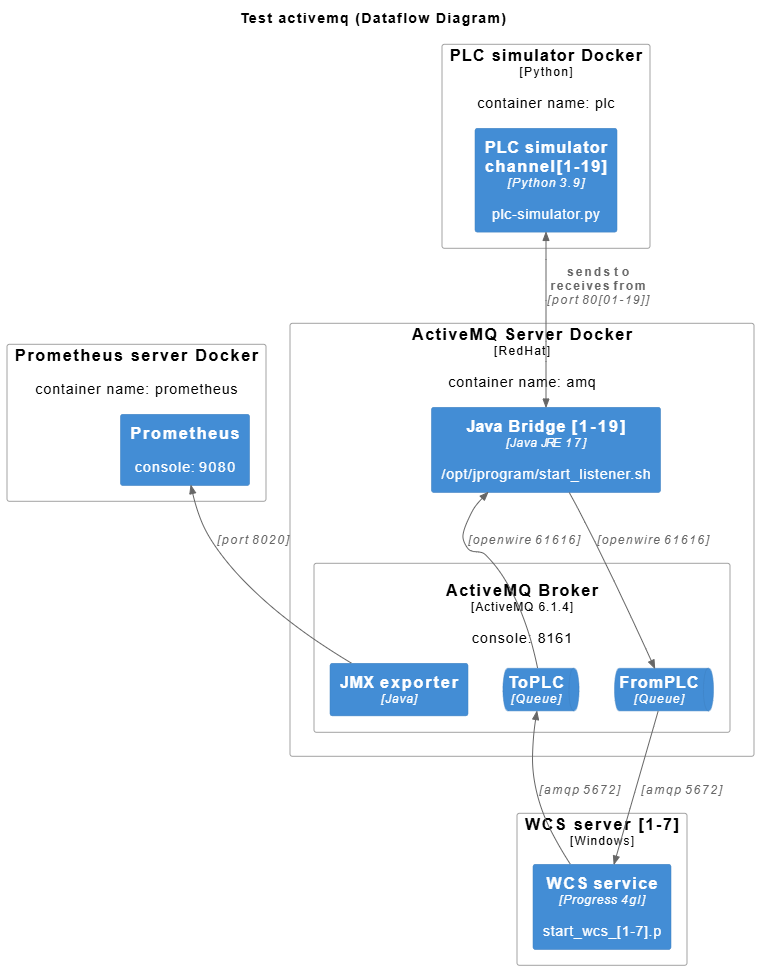
\includegraphics[width=.95\textwidth]{img/test_amq_dataflow.png}
  \caption{\label{fig:test_amq_dataflow}Dataflow test AMQ}
\end{figure}

\subsubsection{Installatie}
Het installeren van dit systeem wordt duidelijk uitgelegd in de officiële documentatie van Apache ActiveMQ.
Configuratie moet aangepast worden in ``activemq.xml'' om de service toegankelijk te maken voor externe services.
Daarnaast moet het bestand ``setenv'' aangepast worden om de metrics via ``jmx\_exporter'' beschikbaar te maken.

\subsubsection{Integratie}
Het WCS-script kan via poort 5672 een AMQP-verbinding tot stand brengen met de ActiveMQ-server.
De Java-listeners op die server zijn een aparte service, maken gebruik van een JMS-library en verbinden via het Openwire-protocol op poort 16161.
\\\\
Om de simulatie zo realistisch mogelijk te maken, zijn er twee queues opgezet. 
Berichten afkomstig van de PLC worden via de gebruikte poort, via de Java-listener naar de queue gestuurd en krijgen daarbij een property genaamd kanaal.
Dankzij deze property kunnen de berichten eenvoudig worden gefilterd op kanaal. 
\\\\
Voor monitoring wordt de jmx\_exporter gebruikt, waarmee de metrics beschikbaar worden gesteld aan externe software zoals Prometheus. 
Deze monitoringdata kan benaderd worden via een zelf te configureren poort, in dit geval poort 8020.

\subsubsection{Performantie}
In deze test worden 19 PLC connecties gemaakt met de Java listeners die elk per 0.1 seconde een bericht versturen naar de  ``FromPLC'' queue.
Hierdoor worden meer dan 1680 berichten per minuut gesimuleerd en wordt er voldaan aan de minimale vereisten op gebied van performantie.
Het opmeten van deze test wordt verdeeld in twee categorieën, dequeued- en enqueued messages.
Om correct de throughput te meten moeten we beide categorieën meten omdat dit de volledige transactie representeert. 
\\\\
Volgende grafiek bevestigd dat er per minuut meer dan 1680 berichten kan geplaatst worden op de twee queues:
\begin{figure}[h!]
  \centering
  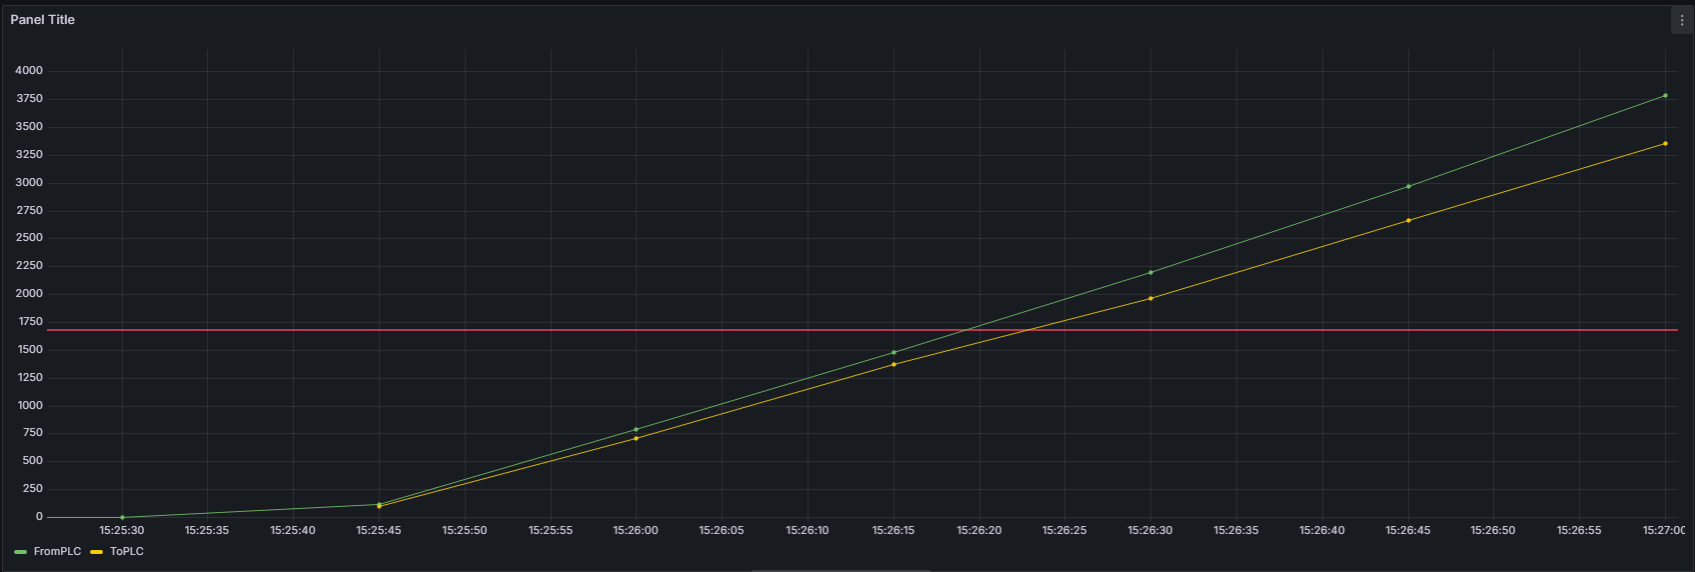
\includegraphics[width=.95\textwidth]{img/amq-enqueue-count.png}
  \caption{\label{fig:amq_enqueue_count}Enqueue ActiveMQ}
\end{figure}
\newpage
Zoals de grafiek laat zien kan de message broker meer dan 1680 berichten naar de consumer versturen van iedere queue binnen één minuut.
\begin{figure}[h!]
  \centering
  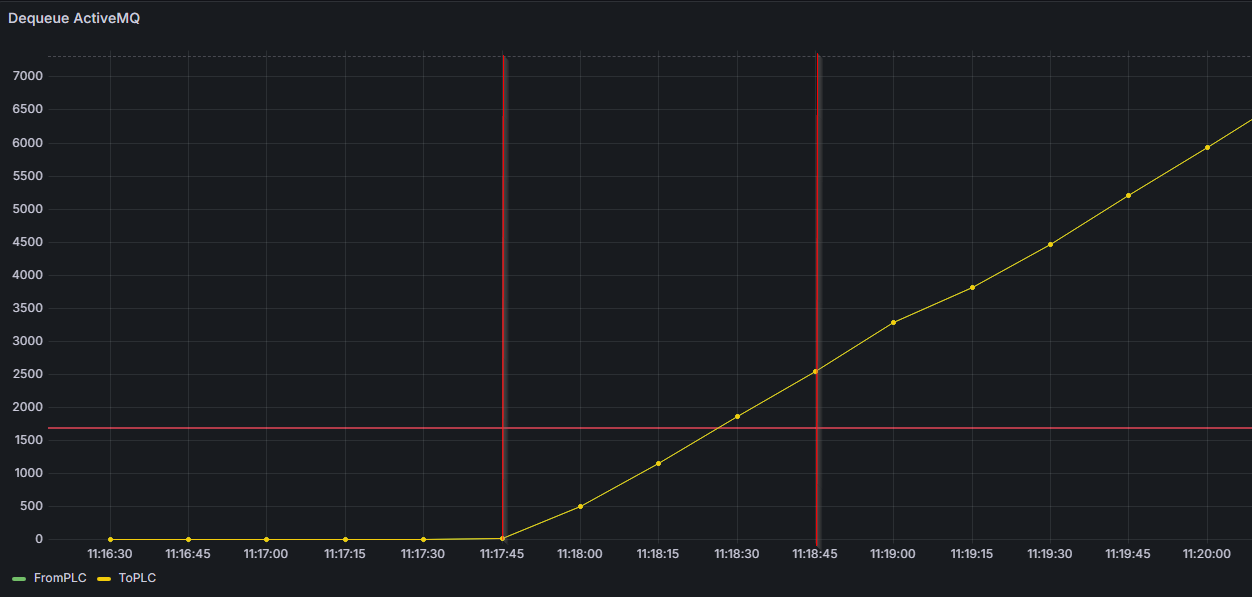
\includegraphics[width=.95\textwidth]{img/amq-dequeue-count.png}
  \caption{\label{fig:amq_dequeue_count}Dequeue ActiveMQ}
\end{figure}

\subsubsection{Samenvatting}
De installatie en integratie kunnen worden uitgevoerd zonder al te complexe aanpassingen, 
wat het proces gebruiksvriendelijk en eenvoudig maakt.
Monitoring is eenvoudig en gemakkelijk toegankelijk. 
Een mooie extra is de admin console die beschikbaar is via ``http://localhost:8161/admin'', waar de metrics kunnen worden geraadpleegd.
Wat betreft prestaties voldoet dit product aan de verwachtingen omdat het meer dan 1680 berichten binnen één minuut kan verwerken via twee queues.

\newpage
\subsection{Test RabbitMQ}
In deze test werd opnieuw een Docker container gemaakt met een RedHat OS instantie, waarop RabbitMQ 
werd geïnstalleerd via een \hyperref[listing:docker_rabbitmq]{DockerFile}.
\\\\
Overzicht infrastructuur:
\begin{figure}[!h]
  \centering
  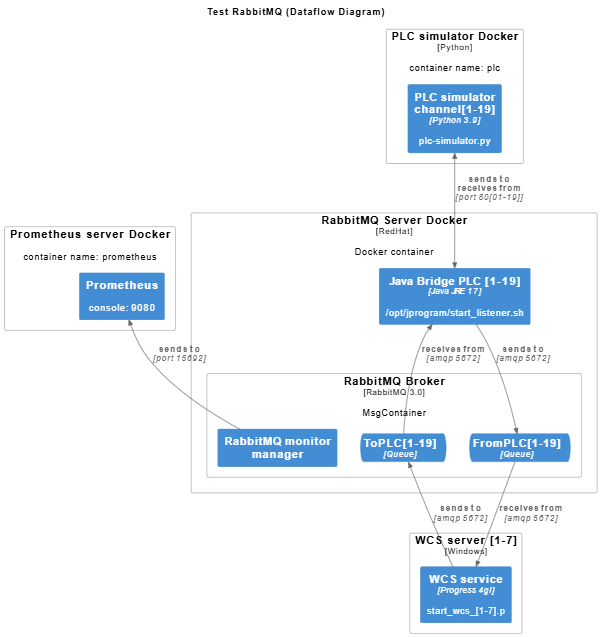
\includegraphics[width=.95\textwidth]{img/test-rabbitmq-dataflow.png}
  \caption{\label{fig:test_rabbitmq_dataflow}Dataflow test RabbitMQ}
\end{figure}

\subsubsection{Installatie}
Deze software heeft een zeer uitgebreide documentatie op de officiële site waardoor het gemakkelijk te installeren is.
RabbitMQ vereist officiële repositories voor uitbreidingen, Erlang runtime en GPG-sleutels om de installatie te verifiëren.
Er is geen configuratie bestand voorzien tijdens de installatie waardoor de originele settings van kracht zijn.
Om deze settings aan te passen is er in de documentatie een voorbeeld \hyperref[sec:config_rabbitmq]{configuratiebestand} voorzien.
De basis configuratie kan met minimale aanpassingen een werkende messaging broker tot stand brengen.
Omdat de configuratie uitgebreid is, kan deze technologie voldoen aan complexe opstellingen.

\subsubsection{Integratie}
Om de Java listeners en het WCS te laten communiceren met de message broker werd gekozen voor het AMQP protocol via het poort 5672.
Monitoring voor Prometheus is voorzien in het RabbitMQ management packet en is bereikbaar via ``http://localhost:15672/''.
Omdat er geen filtering mogelijk is moet er voor ieder kanaal een queue voorzien worden en wijken we af van de opzet van het huidige systeem.
Hierdoor zijn er 38 queues nodig, 19 voor de FromPLC berichten en 19 voor de ToPLC berichten.
\\\\
Berichten kunnen enkel verstuurd worden als binaire data waardoor de inhoud van een bericht eerst moet omgezet worden naar een binary array door de producer.
Ook na het consumeren van een bericht moet deze eerst omgezet worden van binaire data naar het string datatype.

\subsubsection{Performantie}
In deze test worden opnieuw 19 socket connecties gemaakt door het plc script met de Java listeners die elk per 0.1 seconde een bericht versturen naar de relevante queue.
Hierdoor worden meer dan 1680 berichten per minuut verstuurd om te kunnen voldoen aan de minimale vereisten op gebied van performantie.
Het opmeten van deze test wordt verdeeld in twee categorieën, dequeued- en enqueued messages.
Het verschil met vorige test is dat er hier meerdere queues zijn, 19 voor de FromPLC en 19 voor de ToPLC. 

\begin{figure}[h!]
  \centering
  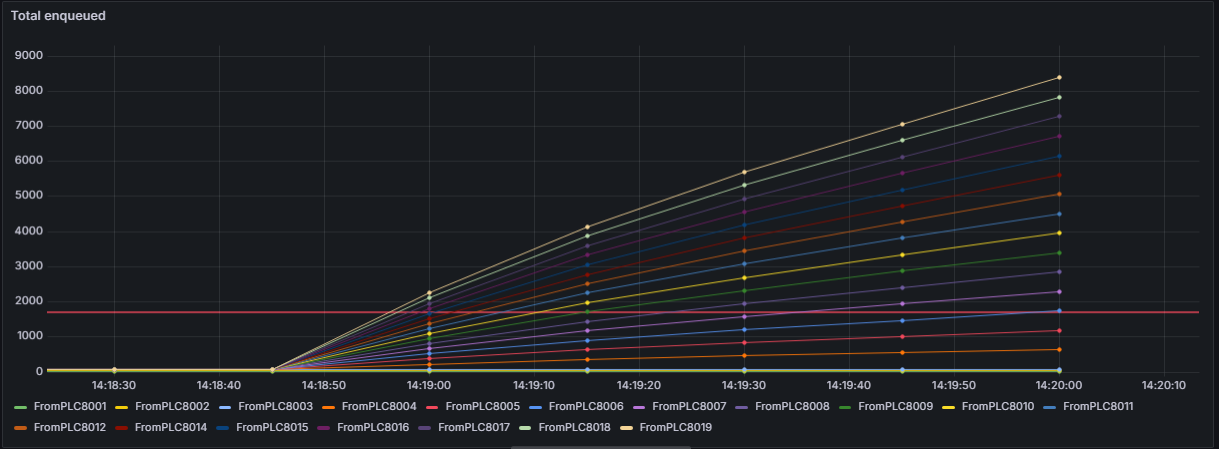
\includegraphics[width=.95\textwidth]{img/rabbitmq-enqueue-count-FromPLC.png}
  \caption{\label{fig:rabbitmq_enqueue_fromplc_count}RabbitMQ enqueue FromPLC}
\end{figure}

\begin{figure}[h!]
  \centering
  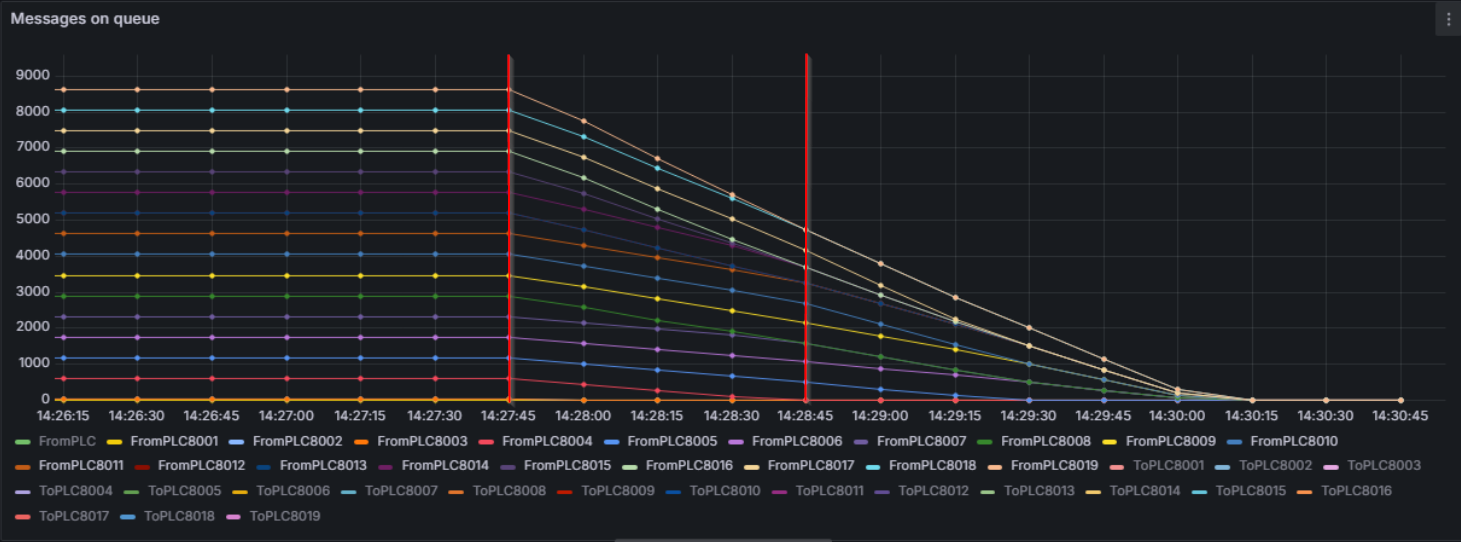
\includegraphics[width=.95\textwidth]{img/rabbitmq-dequeue-count-FromPLC.png}
  \caption{\label{fig:rabbitmq_dequeue_fromplc_count}RabbitMQ dequeue FromPLC}
\end{figure}

\begin{figure}[h!]
  \centering
  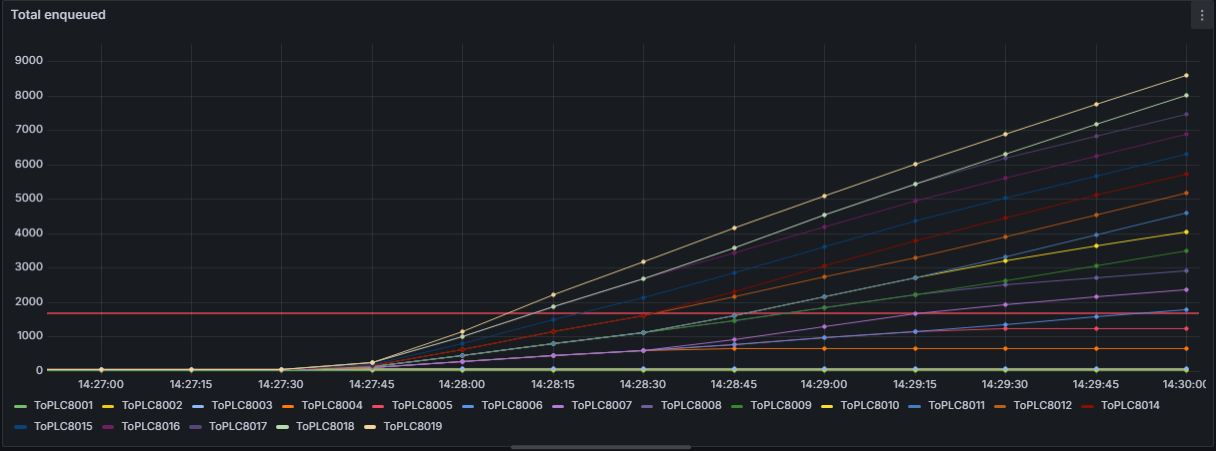
\includegraphics[width=.95\textwidth]{img/rabbitmq-enqueue-count-ToPLC.png}
  \caption{\label{fig:rabbitmq_enqueue_toplc_count}RabbitMQ enqueue ToPLC}
\end{figure}

\begin{figure}[h!]
  \centering
  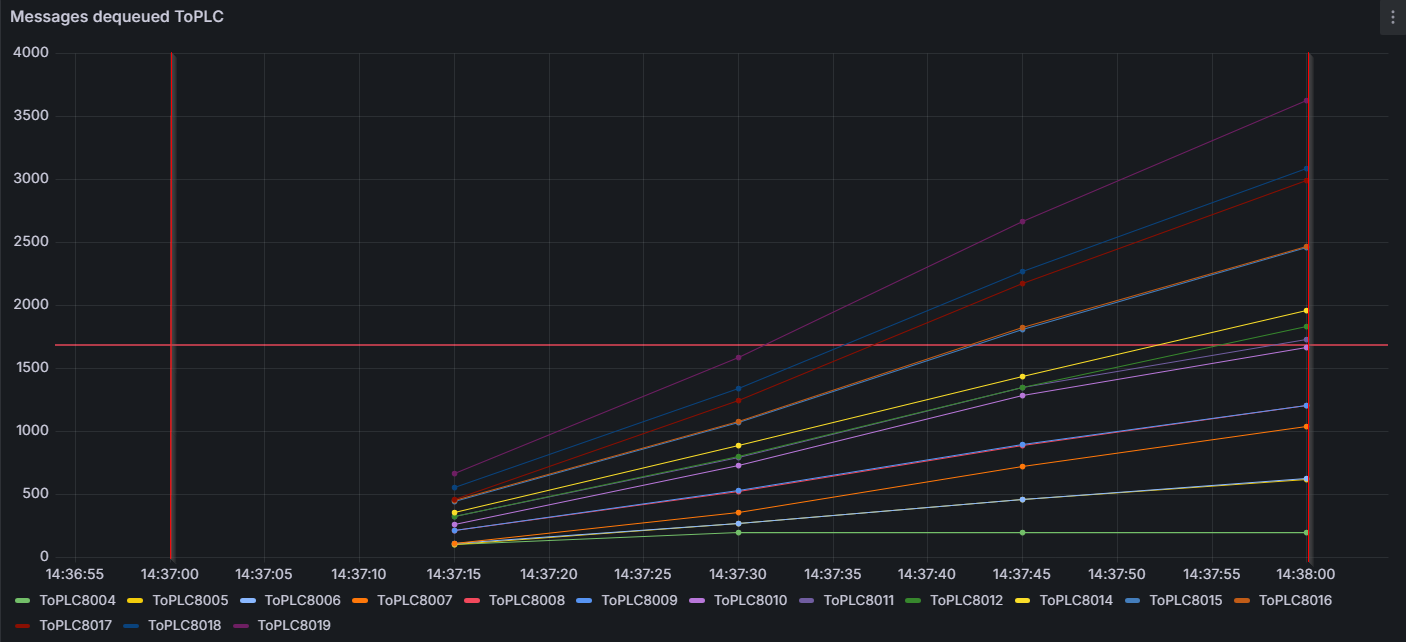
\includegraphics[width=.95\textwidth]{img/rabbitmq-dequeue-count-ToPLC.png}
  \caption{\label{fig:fig:rabbitmq_dequeue_fromplc_count}RabbitMQ dequeue ToPLC}
\end{figure}

\subsubsection{Samenvatting}
RabbitMQ lijkt een goede oplossing dat compatibel is met het huidige systeem, 
maar heeft wel wat aanpassingen nodig omdat filtering niet kan toegepast worden.
Om dit product te gebruiken moet er voor ieder kanaal een aparte queue voorzien worden.
Daarnaast moeten berichten ook omgezet worden en verstuurd worden als binaire data.
\newpage

\subsection{Test Artemis}
In deze test wordt ook een \hyperref[listing:docker_artemis]{Dockerfile} gebruikt voor de installatie.
Overzicht van de infrastructuur:
\begin{figure}[h!]
  \centering
  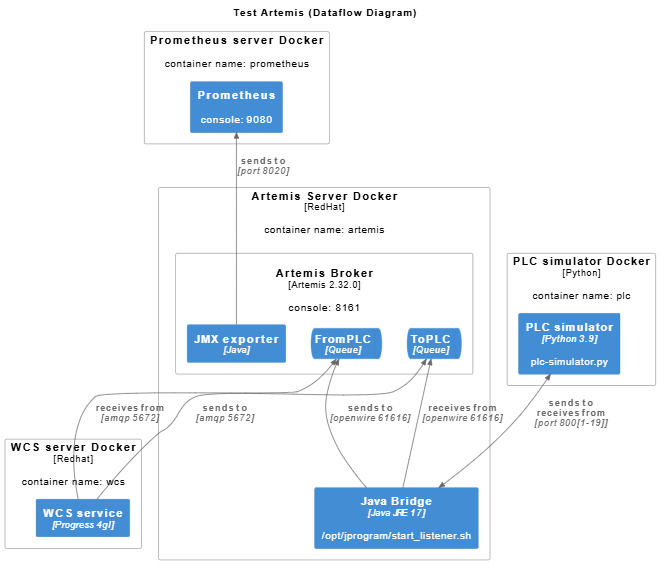
\includegraphics[width=.95\textwidth]{img/test-artemis-dataflow.png}
  \caption{\label{fig:test_artemis_dataflow}Dataflow test Artemis}
\end{figure}

\subsubsection{Installatie}
Het installeren van dit systeem wordt net zoals de andere technologieën duidelijk uitgelegd in de officiële documentatie van Apache.
Configuratie moet hier niet aangepast worden in ``broker.xml'' om de service toegankelijk te maken voor externe services.
Artemis kan verschillende broker instanties opstarten binnen dezelfde JVM, in tegenstelling tot bijvoorbeeld ActiveMQ, dat slechts één instantie kan starten.

\subsubsection{Integratie}
Om de metrics aan te bieden kan je een artemis-prometheus plugin downloaden en toevoegen in de installatie.
Hiervoor moet de \hyperref[listing:broker_artemis]{``broker.xml''} aangepast worden met het toevoegen van de metrics plugin.
deze maakt de metrics toegankelijk via een webpagina.
Hiervoor moet de plugin gecompileerd worden zodat de ``metrics.war'' in de web folder van actieve broker kan geplaatst worden.
Om de webpagina beschikbaar te maken moet de \hyperref[listing:bootstrap_artemis]{``bootstrap.xml''} aangepast worden.

\subsubsection{Performantie}
In deze test worden 19 PLC connecties gemaakt met de Java listeners die elk per 0.1 seconde een bericht versturen naar de ``FromPLC'' queue.
Hierdoor worden meer dan 1680 berichten per minuut verstuurd en wordt er voldaan aan de minimale vereisten op gebied van performantie.
Het opmeten van deze test wordt verdeeld in twee categorieën, dequeued- en enqueued messages.
Om correct de throughput te meten moeten we beide categorieën meten omdat dit de volledige transactie representeert. 
\\\\
Volgende grafiek geeft weer hoeveel berichten er per minuut verzonden kunnen worden naar de message queue.
\begin{figure}[h!]
  \centering
  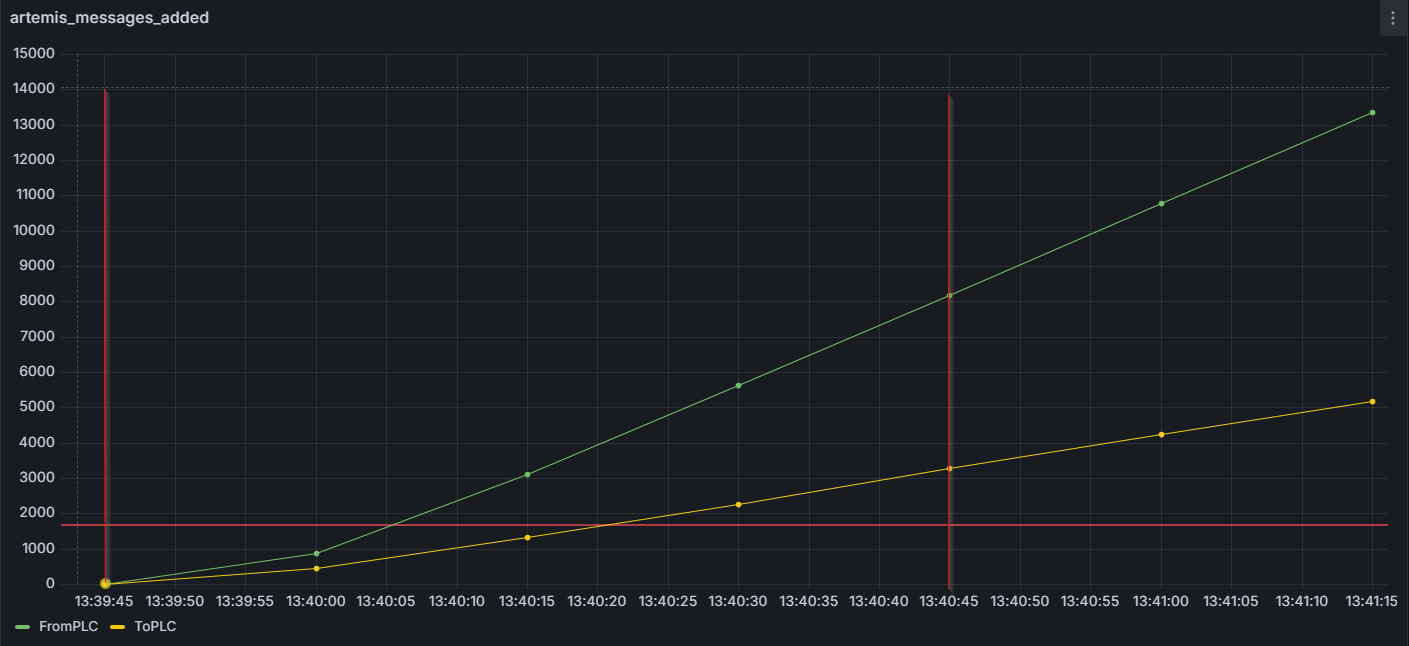
\includegraphics[width=.95\textwidth]{img/artemis-enqueue-count.png}
  \caption{\label{fig:artemis_enqueue_count}Enqueue Artemis}
\end{figure}

\begin{figure}[h!]
  \centering
  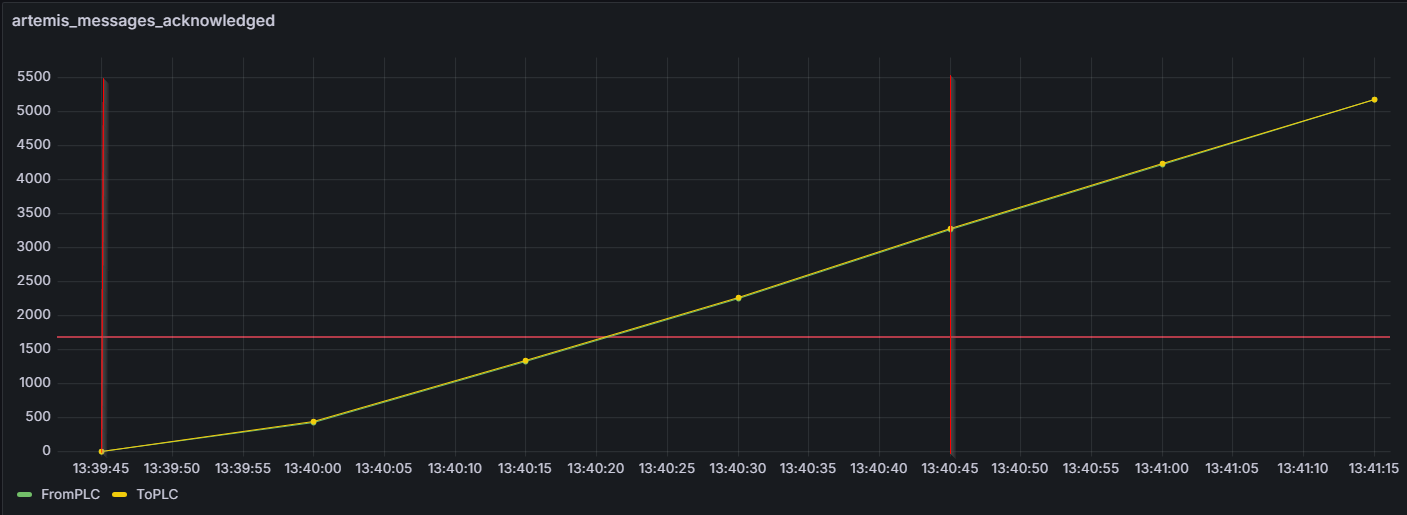
\includegraphics[width=.95\textwidth]{img/artemis-dequeue-count.png}
  \caption{\label{fig:artemis_dequeue_count}Dequeue Artemis}
\end{figure}

\subsubsection{Samenvatting}
De installatie en integratie kunnen worden uitgevoerd zonder al te complexe aanpassingen, 
wat het proces gebruiksvriendelijk en eenvoudig maakt.
Het voorzien van monitoring is evenals eenvoudig en gemakkelijk toegankelijk. 
De admin console is beschikbaar via ``http://localhost:8161'' en is gebruiksvriendelijk en uitgebreider dan de admin console van ActiveMQ Classic.
Wat betreft prestaties voldoet dit product aan de verwachtingen omdat het meer dan 1680 PLC berichten binnen één minuut kan verwerken.

% Voeg hier je eigen hoofdstukken toe die de ``corpus'' van je bachelorproef
% vormen. De structuur en titels hangen af van je eigen onderzoek. Je kan bv.
% elke fase in je onderzoek in een apart hoofdstuk bespreken.

%\input{...}
%\input{...}
%...

%%=============================================================================
%% Conclusie
%%=============================================================================

\chapter{Conclusie}%
\label{ch:conclusie}

% TODO: Trek een duidelijke conclusie, in de vorm van een antwoord op de
% onderzoeksvra(a)g(en). Wat was jouw bijdrage aan het onderzoeksdomein en
% hoe biedt dit meerwaarde aan het vakgebied/doelgroep? 
% Reflecteer kritisch over het resultaat. In Engelse teksten wordt deze sectie
% ``Discussion'' genoemd. Had je deze uitkomst verwacht? Zijn er zaken die nog
% niet duidelijk zijn?
% Heeft het onderzoek geleid tot nieuwe vragen die uitnodigen tot verder 
%onderzoek?

De drie kandidaten die aan de testen werden onderworpen, voldeden allemaal aan de vooraf gestelde eisen.
Tussen deze kandidaten zijn duidelijke verschillen te merken waardoor één kandidaat als optimale message broker kan gekozen worden.

\section{Apache ActiveMQ}
Apache ActiveMQ Classic is een snelle en kortetermijnoplossing, 
omdat deze met minimale aanpassingen eenvoudig te integreren is in het huidige systeem.

\section{RabbitMQ}
RabbitMQ is een modern messaging-systeem dat zowel toekomstbestendig als zeer krachtig is. 
In tegenstelling tot ActiveMQ en Artemis, biedt RabbitMQ geen ingebouwde filtering, wat het minder geschikt kan maken voor de huidige opstelling.
RabbitMQ heeft een grote community en wordt het actief ontwikkeld. Het kan een robuuste oplossing zijn, 
mits de huidige opstelling wordt aangepast.

\section{Apache Artemis}
Apache Artemis komt naar voor als beste van de drie kandidaten:
\begin{itemize}
    \item \textbf{Performantie:} Uit de performantie resultaten blijkt dat Artemis duidelijk sneller is dan ActiveMQ
    \item \textbf{Functionaliteit:} Filtering kan toegepast worden in tegenstelling tot RabbitMQ.
    \item \textbf{Toekomstbestendig} Als modernere versie van ActiveMQ is Artemis beter geschikt voor langdurig gebruik.
    \item \textbf{Implementatiegemak:} Vereist minimale aanpassingen om te integreren in tegenstelling tot RabbitMQ.
    \item \textbf{Schaalbaarheid:} Het systeem ondersteunt meerdere instanties, wat meer schaalbaarheid biedt dan ActiveMQ.
\end{itemize}  

\section{Conclusie}
Hoewel alle kandidaten voldoen aan de gestelde eisen, biedt Apache Artemis de beste balans tussen prestaties, 
functionaliteit, schaalbaarheid en implementatiegemak. 
Dit maakt het de meest geschikte keuze voor zowel de huidige als toekomstige behoeften.





%---------- Bijlagen -----------------------------------------------------------

\appendix

\chapter{Onderzoeksvoorstel}

Het onderwerp van deze bachelorproef is gebaseerd op een onderzoeksvoorstel dat vooraf werd beoordeeld door de promotor. Dat voorstel is opgenomen in deze bijlage.

%% TODO: 
%\section*{Samenvatting}

% Kopieer en plak hier de samenvatting (abstract) van je onderzoeksvoorstel.

% Verwijzing naar het bestand met de inhoud van het onderzoeksvoorstel
%---------- Inleiding ---------------------------------------------------------

% TODO: Is dit voorstel gebaseerd op een paper van Research Methods die je
% vorig jaar hebt ingediend? Heb je daarbij eventueel samengewerkt met een
% andere student?
% Zo ja, haal dan de tekst hieronder uit commentaar en pas aan.

\paragraph{Opmerking}

Dit voorstel is gebaseerd op het onderzoeksvoorstel dat werd geschreven in het
kader van het vak Research Methods dat ik vorig academiejaar heb
uitgewerkt.

\section{Inleiding}%
\label{sec:inleiding}

\subsection{Overzicht}
Grote bedrijven hebben meestal een complexe bedrijfsstructuur, wat wil zeggen dat er verschillende 
domeinen en subdomeinen met specifieke doeleinden binnen de organisatie de steunpilaren vormen om de bedrijvigheid mogelijk te maken. 
Voorbeeld hiervan is e-commerce dat de klant de mogelijkheid geeft een bestelling te plaatsen, 
magazijnbeheer (WMS) om de voorraad te beheren, aankoop om onderdelen te bestellen bij de leverancier en transport (TMS) 
om die onderdelen tot bij de klant te krijgen. 
\newline 

Om deze taken te kunnen uitvoeren wordt er gebruik gemaakt van één of meerdere \emph{services} die de vooropgestelde 
functionaliteiten van een subdomein supporteert. 
% hook
In de IT terminologie heet deze opstelling \emph{“Service oriented architecture” (SOA)} 
en wordt deze steeds populairder omdat dit voordelig is voor de \emph{flexibiliteit} en \emph{schaalbaarheid} \autocite{Bellemare2020}.
\newline 

Door deze onderlinge afhankelijkheid moeten services met elkaar kunnen communiceren.
Om dit mogelijk te maken, zijn verschillende \emph{messaging systemen} beschikbaar op de markt, 
die elk hun eigenschappen en toepassingen hebben. 
\newline 

\subsection{Probleemstelling}
Het bedrijf dat onderwerp is in dit onderzoek, bevindt zich in een fase van digitale transformatie 
waarbij het monolithisch legacy systeem wordt opgesplitst in componenten, genaamd \emph{services}, 
die zowel in de cloud als op lokale (on-premise) systemen draaien. Daarnaast heeft het bedrijf een snelle groei 
doorgemaakt zonder algemene afspraken te maken rond het gebruik van messaging systemen. Dit heeft geresulteerd in de 
implementatie van verschillende messaging systemen, waardoor er een diversiteit aan oude en moderne technologieën in gebruik is. 
Door de vele nieuwe \emph{services} die naast de bestaande zijn ontstaan en de snelle veranderingen in technologie, 
is er een dringende behoefte om de gebruikte communicatiemiddelen te herzien. 
\newline

De nadelen van te veel verschillende messaging systemen zijn onder andere de onderhoudskosten, wat betekent 
dat mensen in de firma opgeleid moeten worden om die te onderhouden. 
Hierdoor komt de efficiëntie in het gedrang op vlak van het uitrollen en onderhouden van de verschillende systemen.
\newline 

\subsection{Onderzoeksdoelstelling}
Het doel van dit onderzoek is om na te gaan welk messaging systeem het meest optimaal is binnen de organisatie. 
Hierbij moet er rekening gehouden worden met de verschillende subdomeinen, die elk hun eigenschappen en \newline non-functional requirements 
hebben, zoals flexibiliteit, performantie, beveiliging en schaalbaarheid.
Naast de vergelijkende studie moet er ook gekeken worden wat de kosten en de inspanningen zijn 
voor het integreren van een gekozen messaging systeem. \newline 

Het belang van een consistent gebruik van de meest optimale technologie is op lange termijn
een goede aanwinst voor het bedrijf. 

\subsection{Onderzoeksvraag en deelvragen}

Welke \emph{messaging technologieën} zijn optimaal voor het bedrijf en zijn subdomeinen?
Enkele cruciale deelvragen met betrekking tot de hoofdvraag:

\begin{enumerate}
  \item Waarom is een weloverwogen keuze van essentieel belang?
  \item Welke messaging systemen zijn er beschikbaar?
  \item Wat zijn hun kenmerken en voordelen?
  \item Wat is de inspanning om een gekozen technologie te implementeren?
  \item Wat zijn de non-functional requirements zijn er vanuit de bestaande services?
  \item Welke systeem is een weloverwogen keuze?
\end{enumerate}

\subsection{Opbouw van het onderzoek}
Eerst zal de literatuurstudie in hoofdstuk \ref{sec:literatuurstudie} het concept 
van een domein in de bedrijfscontext toe lichten;
de relatie met \emph{Microservices} in kaart gebracht; 
de relevantie en verschillen tussen synchrone en asynchrone communicatie vergeleken; 
de rol van een messaging systeem binnen de IT-infrastructuur besprokenen tot slot 
uitgelegd waarom een weloverwogen keuze van essentieel belang is.

Hoofdstuk \ref{sec:methodologie} beschrijft de methodologie en de stappen die nodig zijn om dit onderzoek te ondersteunen
en te leiden tot een rapport met aanbevelingen. 

In hoofdstuk \ref{sec:verwachte-resultaten} worden de verwachte resultaten beschreven, gevolgd door 
hoofdstuk \ref{sec:discussie-conclusie} met de verwachte conclusie van het onderzoek.

\bigskip


%---------- Stand van zaken (State-of-the-art)---------------------------------------------------

\section{Literatuurstudie}%
\label{sec:literatuurstudie}

% Hier beschrijf je de \emph{state-of-the-art} rondom je gekozen onderzoeksdomein, d.w.z.\ een inleidende, doorlopende tekst over het onderzoeksdomein van je bachelorproef. Je steunt daarbij heel sterk op de professionele \emph{vakliteratuur}, en niet zozeer op populariserende teksten voor een breed publiek. Wat is de huidige stand van zaken in dit domein, en wat zijn nog eventuele open vragen (die misschien de aanleiding waren tot je onderzoeksvraag!)?

% Je mag de titel van deze sectie ook aanpassen (literatuurstudie, stand van zaken, enz.). Zijn er al gelijkaardige onderzoeken gevoerd? Wat concluderen ze? Wat is het verschil met jouw onderzoek?

% Verwijs bij elke introductie van een term of bewering over het domein naar de vakliteratuur, bijvoorbeeld~\autocite{Hykes2013}! Denk zeker goed na welke werken je refereert en waarom.

% Draag zorg voor correcte literatuurverwijzingen! Een bronvermelding hoort thuis \emph{binnen} de zin waar je je op die bron baseert, dus niet er buiten! Maak meteen een verwijzing als je gebruik maakt van een bron. Doe dit dus \emph{niet} aan het einde van een lange paragraaf. Baseer nooit teveel aansluitende tekst op eenzelfde bron.

% Als je informatie over bronnen verzamelt in JabRef, zorg er dan voor dat alle nodige info aanwezig is om de bron terug te vinden (zoals uitvoerig besproken in de lessen Research Methods).

% Voor literatuurverwijzingen zijn er twee belangrijke commando's:
% \autocite{KEY} => (Auteur, jaartal) Gebruik dit als de naam van de auteur
%   geen onderdeel is van de zin.
% \textcite{KEY} => Auteur (jaartal)  Gebruik dit als de auteursnaam wel een
%   functie heeft in de zin (bv. ``Uit onderzoek door Doll & Hill (1954) bleek
%   ...'')

% Je mag deze sectie nog verder onderverdelen in subsecties als dit de structuur van de tekst kan verduidelijken.

\bigskip
 
\subsection{Definitie van Domein}
Zoals de titel van deze paper aangeeft is het bedrijf een complex bedrijf dat verschillende domeinen en subdomeinen bevat.
Het woord domein in de bedrijfscontext is een probleemgebied waar een bedrijf zich op richt en oplossingen voor biedt. 
De firma heeft als hoofddomein e-commerce en omvat alle aspecten van hun online retailactiviteiten, 
zoals het beheren van producten, het verwerken van bestellingen, klantenservice, marketing en logistiek.
\newline 

Een domein bevat subdomeinen die elk gericht zijn op een specifieke subset zoals bijvoorbeeld ``Productcatalogus''.
Dit subdomein richt zich specifiek op het beheren van productinformatie, met ondersteuning van het toevoegen, bewerken en verwijderen van producten, 
evenals het bijhouden van voorraadniveaus en prijzen.
\newline 

Een subdomein kan dus worden beschouwd als een stukje van het domein, 
dat net als het domein zelf behoort tot het probleemgebied.   
Terwijl een domein een breed probleemgebied beschrijft, bevat een subdomein een specifieke afbakening, genaamd \emph{bounded context}.
Dit maakt het mogelijk om \emph{microservices} binnen deze afbakening te ontwikkelen en te beheren \autocite{Bellemare2020}.

\subsection{Definitie van Microservices}
\emph{Microservices} zijn onafhankelijk inzetbaar en richten zich op specifieke aspecten van een 
subdomein binnen een \emph{bounded context}. 
Dit concept valt onder ``Domain-driven design'' en vertegenwoordigt een stijl van \emph{``Loose coupling''}, 
wat wil zeggen dat het in theorie autonoom kan functioneren.
Binnen de \emph{bounded context} zijn de interne onderdelen, zoals code en dataschema's, aan elkaar gekoppeld maar ze zijn nooit verbonden 
aan iets buiten die context, zoals een database of klassedefinitie van een ander context. 
Dit stelt elke service in staat om alleen te definiëren wat het nodig heeft in plaats van andere elementen te gebruiken uit andere services.
Om gegevens en informatie uit te wisselen tussen deze verschillende domeinen communiceren ze met elkaar over het netwerk, 
zoals via RESTful API's of messaging queues. 
Het primaire doel van de \emph{microservice-architectuur} is flexibiliteit, maar daarnaast brengt het ook voordelen voor developers, 
zoals een betere samenwerking zonder elkaar in de weg te zitten. 
Ontwikkelaars gaan ook hun deel van het systeem beter begrijpen, omdat ze zich kunnen 
concentreren op de specifieke kennis van hun service.
\emph{Microservices} zijn dus een type van \emph{Service-oriented architecture (SOA)} en weerspiegelt een duidelijke mening over hoe een 
service zijn grenzen moet afbakenen ~\autocite{Newman2020}.
\newline

\begin{figure}[H]
  \centering
  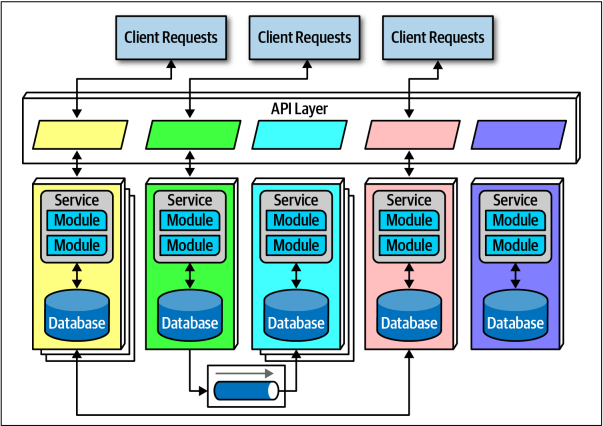
\includegraphics[width=.5\textwidth]{topology-microservices.png}
  \caption{\label{fig:img}Toplology of the Microservices Architecture style \autocite[figure 17 - 1]{MarkRichards2021}.}
\end{figure}

%\subsection{Soorten communicatie}
% file:///C:/Data/Downloads/IJMECS-V12-N2-5.pdf
 
\subsection{Synchroon vs. asynchroon}
In de wereld van microservices communiceren services zowel \emph{synchroon} als \emph{asynchroon} en spelen deze benaderingen een cruciale rol, 
elk met hun eigen voor- en nadelen. \emph{Synchrone microservices} werken volgens een direct 
afhankelijkheidsmodel, omdat services met elkaar communiceren in een vraag-antwoordpatroon. 
Deze synchrone communicatie kan leiden tot ingewikkelde onderlinge afhankelijkheden, vertragingen en complexiteiten bij het debuggen 
van de logica. Bovendien wordt het schalen van synchrone microservices uitdagend, 
aangezien de schaalbaarheid van één service sterk afhankelijk is van andere services die het gebruikt \autocite{Bellemare2020}. 
\newline

Daartegenover bieden \emph{asynchrone microservices} een reeks voordelen. Ze bieden grotere schaalbaarheid, technologische 
flexibiliteit en aanpassingsvermogen aan veranderende zakelijke vereisten. 
In plaats van de synchrone manier van communicatie zijn \emph{asynchrone microservices} 
gemakkelijker te herstructureren en te onderhouden. 
Ze vergemakkelijken \emph{continuous delivery} door hun onafhankelijkheid omdat de communicatie 
met een \emph{messaging systeem} opgevangen wordt. Hun verminderde afhankelijkheden en 
geïsoleerde karakter maken het testen relatief eenvoudiger en robuuster.
Het enige grote nadeel in asynchrone communicatie is \emph{error handling}, 
omdat dit niet opgevangen kan worden door de verzendende partij.
\newline

\begin{figure}[H]
  \centering
  \includegraphics[width=.5\textwidth]{synchronous_vs_async_calls.png}
  \caption{\label{fig:img}Synchronous versus asynchronous communication \autocite[figure 14 -- 13]{MarkRichards2021}.}
\end{figure}

In praktische termen is het vinden van de juiste balans tussen synchrone en \emph{asynchrone microservices} cruciaal, 
afhankelijk van de specifieke behoeften van een organisatie en de aard van haar bedrijfsprocessen. 
Een hybride aanpak waarin beide architecturen naast elkaar bestaan en elkaar aanvullen blijkt vaak de meest effectieve strategie te zijn. 
Deze aanpak stelt organisaties in staat om de sterke punten van zowel synchrone als asynchrone modellen te benutten, 
waardoor flexibiliteit, schaalbaarheid en onderhoudsgemak worden gegarandeerd in complexe \newline IT-landschappen.
In deze paper ligt de focus op \emph{asynchrone communicatie} voor het gebruik van \emph{messaging systemen}.
\newline

\subsection{Overzicht Messaging Systeem}
Messaging systemen hebben dus een asynchrone werking en vallen onder \newline \emph{Inter-Process Communication (IPC)}. 
Deze systemen zijn \emph{socket-based} en maken gebruik van \emph{Message Queuing}, dat de \emph{publish-subscribe} of de \emph{point-to-point} methodiek gebruikt \autocite{Dinari2020}. 
\newline
Een socketverbinding maakt gebruik van een endpoint gespecificeerd met een IP-adres en een \newline poortnummer, 
waarmee twee autonome processen verbonden zijn, hetzij op dezelfde, hetzij op verschillende machines.
\newline
\emph{Message Queuing} gebruikt deze manier van verbinden en maakt het voor applicaties mogelijk om asynchroon 
te communiceren zonder te moeten wachten op een antwoord van de ontvanger. 
Er zijn twee methodieken in deze systemen. 
\newline
\newline

De eerste methodiek is \emph{publish-subscribe}, waarbij de zender, genaamd \emph{publisher} niet verantwoordelijk is voor het beheer 
en het rechtstreeks verzenden van de berichten naar specifieke ontvangers, die \emph{subscribers} of abonnees worden genoemd. 
In plaats daarvan worden berichten door het messaging systeem of broker geclassificeerd en ter 
beschikking gesteld van de subscribers die ingetekend hebben op berichten uit een specifieke klasse.
Vervolgens ontvangen \emph{subscribers} berichten uit de klassen die voor hen interessant zijn, zonder dat ze kennis hebben van de \emph{publishers}.
Met het \emph{publish-subscribe-model} specificeert de afzender nooit expliciet de ontvanger,
hij weet zelfs niet of er wel of geen ontvanger bestaat.
\newline

\begin{figure}[h]
  \centering
  \includegraphics[width=.4\textwidth]{fig1-publish-subscribe.png}
  \caption{\label{fig:img}Publisher-Subscriber system\autocite{Sharvari2019}.}
\end{figure}

In dit model ontvangen \emph{subscribers} slechts een subset van de totale gepubliceerde berichten. 
Het proces van het selecteren en verwerken van de berichten wordt filtering genoemd. 
Er zijn twee vormen van filtering: op basis van onderwerp (topic) en op basis van inhoud (content).
\newline

In een op \emph{topic} gebaseerd systeem worden berichten geplaatst in \emph{topics} wat logische kanalen zijn.
\emph{Subscribers} ontvangen berichten van de \emph{topics} waarop ze zich hebben geabonneerd.
Alle \emph{subscribers} ontvangen dezelfde berichten uit dezelfde \emph{topics}. 
Deze methode zorgt voor een \emph{one-to-many} vorm van communicatie.
\newline

De tweede methodiek genaamd point-to-point gebruikt \emph{queuing} waarbij de \emph{producer} berichten plaatst in een specifieke queue, 
waarna een \emph{consumer} de berichten uitleest in een sequentiele volgorde. 
Met andere woorden, een bericht wordt slechts aan één \emph{consumer} bezorgt.

\newpage

\subsection{Het belang van een optimale \newline messaging technologie}

In het artikel ``Too Much Middleware'' betoogt \textcite{Stonebraker2002} dat de overvloed aan middleware systemen, 
waaronder applicatieservers, workflowproducten, integratie systemen en \newline ETL-systemen heeft geleid tot een gefragmenteerd landschap 
met overlappende functionaliteit. 
Deze diversiteit creëert complexiteit en inefficiëntie voor bedrijven. 
\textcite{Stonebraker2002} stelt dat aanzienlijke consolidatie nodig is en presenteert verschillende manieren waarop dit kan worden bereikt.
\newline

Een aantal onderzoeksvragen uit de probleemstelling dat deels kan worden beantwoord:

\begin{enumerate}

\item \textbf{Waarom is een weloverwogen keuze van essentieel belang?}
  \begin{itemize}
      \item Een weloverwogen keuze is essentieel omdat de huidige overvloed aan middleware systemen complexiteit introduceert en 
      inefficiëntie veroorzaakt. Door zorgvuldig te kiezen en te consolideren kunnen bedrijven deze problemen verminderen en een 
      efficiënter IT-landschap creëren.
  \end{itemize}

\item \textbf{Wat is de inspanning om een gekozen technologie te implementeren?}
  \begin{itemize}
      \item De inspanning om een gekozen technologie te implementeren kan variëren afhankelijk van de specifieke systeemvereisten, 
      de complexiteit van de bedrijfsprocessen en de beschikbare middelen binnen de organisatie. Dit kan onder meer het configureren, 
      aanpassen en integreren van de gekozen technologie omvatten, evenals het trainen van personeel en het uitvoeren van migraties van 
      bestaande systemen.
  \end{itemize}
\end{enumerate}

\newpage

%---------- Methodologie ------------------------------------------------------
\section{Methodologie}%
\label{sec:methodologie}

% Hier beschrijf je hoe je van plan bent het onderzoek te voeren. Welke onderzoekstechniek ga je toepassen om elk van je onderzoeksvragen te beantwoorden? Gebruik je hiervoor literatuurstudie, interviews met belanghebbenden (bv.~voor requirements-analyse), experimenten, simulaties, vergelijkende studie, risico-analyse, PoC, \ldots?

% Valt je onderwerp onder één van de typische soorten bachelorproeven die besproken zijn in de lessen Research Methods (bv.\ vergelijkende studie of risico-analyse)? Zorg er dan ook voor dat we duidelijk de verschillende stappen terug vinden die we verwachten in dit soort onderzoek!

% Vermijd onderzoekstechnieken die geen objectieve, meetbare resultaten kunnen opleveren. Enquêtes, bijvoorbeeld, zijn voor een bachelorproef informatica meestal \textbf{niet geschikt}. De antwoorden zijn eerder meningen dan feiten en in de praktijk blijkt het ook bijzonder moeilijk om voldoende respondenten te vinden. Studenten die een enquête willen voeren, hebben meestal ook geen goede definitie van de populatie, waardoor ook niet kan aangetoond worden dat eventuele resultaten representatief zijn.

% Uit dit onderdeel moet duidelijk naar voor komen dat je bachelorproef ook technisch voldoen\-de diepgang zal bevatten. Het zou niet kloppen als een bachelorproef informatica ook door bv.\ een student marketing zou kunnen uitgevoerd worden.

% Je beschrijft ook al welke tools (hardware, software, diensten, \ldots) je denkt hiervoor te gebruiken of te ontwikkelen.

% Probeer ook een tijdschatting te maken. Hoe lang zal je met elke fase van je onderzoek bezig zijn en wat zijn de concrete \emph{deliverables} in elke fase?

\section{Methodologie}%
\label{sec:methodologie}

Het volgende stappenplan zal helpen om de vergelijkende studie op een verfijnde manier uit te voeren.
Eerst worden de requirements rond messaging systemen per subdomein opgelijst aan de hand van diepte interviews 
met de ontwikkelaars en de software architects. 
Deze requirements zullen ook duidelijk maken welke criteria exact van belang zijn.
Daarnaast worden de verschillende soorten messaging systemen die beschikbaar zijn op de markt opgezocht, bestudeerd en opgelijst in een longlist.
Voor het bekomen van een shortlist zal de longlist onderworpen worden aan eerder opgestelde criteria.
\newline

Tijdens deze studie worden een aantal testen opgesteld om na te gaan of de gekozen technologieën in de shortlist voldoen aan de non-functional requirements.
Na het uitvoeren van de testen zal een uitgebreide analyse uitwijzen welk systeem het meest optimaal is binnen de firma.

\subsection{Stappen plan}

\begin{figure}[htbp]
  \centering
  \begin{tikzpicture}[node distance=1.5cm]
      % Nodes
      \node (start) [rectangle, draw, text width=5cm, align=center] {Requirements verzamelen};
      \node (longlist) [rectangle, draw, below of=start, text width=5cm, align=center] {Long list};
      \node (criteria) [rectangle, draw, below of=longlist, text width=5cm, align=center] {Criteria vaststellen};
      \node (testscenario) [rectangle, draw, below of=criteria, text width=5cm, align=center] {Testscenario's opstellen};
      \node (testen) [rectangle, draw, below of=testscenario, text width=5cm, align=center] {Testen uitvoeren};
      \node (analyseren) [rectangle, draw, below of=testen, text width=5cm, align=center] {Resultaten analyseren};
      \node (rapportage) [rectangle, draw, below of=analyseren, text width=5cm, align=center] {Rapportage en aanbevelingen};

      % Arrows
      \draw [->] (start) -- (longlist);
      \draw [->] (longlist) -- (criteria);
      \draw [->] (criteria) -- (testscenario);
      \draw [->] (testscenario) -- (testen);
      \draw [->] (testen) -- (analyseren);
      \draw [->] (analyseren) -- (rapportage);
  \end{tikzpicture}
  \caption{Stappen van het onderzoeksproces}
  \label{fig:flowchart}
\end{figure}


\bigskip

\subsection{Tijdlijn}

De volgende tijdlijn geeft naar schatting een overzicht van wanneer elk onderdeel zal plaatsvinden en hoeveel tijd elk onderdeel in beslag zal nemen. 
Er zijn vier dagen per maand beschikbaar waarop acht uur kan worden gewerkt aan dit onderzoek.

\newcommand{\ytl}[2]{
  \parbox[b]{8em}{\hfill{\color{cyan}\bfseries\sffamily #1}~$\cdots\cdots$~}\makebox[0pt][c]{$\bullet$}\vrule\quad \parbox[c]{4.5cm}{\vspace{7pt}\color{red!40!black!80}\raggedright\sffamily #2.\\[7pt]}\\[-3pt]
}

\begin{figure}[htbp]
  \centering  
  \rule{\linewidth}{1pt}
  \ytl{Okt, 4 dagen}{Requirements verzamelen -- Criteria vaststellen}
  \ytl{Nov, 4 dagen}{Long list}
  \ytl{Dec, 4 dagen}{Long list}
  \ytl{Jan, 4 dagen}{Opstellen testscenario's}
  \ytl{Feb, 4 dagen}{Opstellen testscenario's}
  \ytl{Mar, 4 dagen}{Testen}
  \ytl{Apr, 4 dagen}{Testen}
  \ytl{Mei, 4 dagen}{Analyseren resultaten}
  \ytl{Jun, 4 dagen}{Rapportage}
  \rule{\linewidth}{1pt}
  \caption{Tijdlijn onderzoek}
  \label{fig:timeline}
\end{figure}

 
\subsection{Requirements verzamelen per \newline subdomein}
In deze stap worden de criteria opgenomen om de longlist in een latere fase te kunnen filteren.
Door de domein architecten en product owners te interviewen en intern documentatie op te zoeken kan een 
lijst met criteria gecategoriseerd worden volgens de non-functional requirements.

\subsection{Evaluatiecriteria vaststellen}
We stellen criteria vast om de verschillende messaging systemen te kunnen evalueren. 
Deze criteria moeten relevant zijn voor de behoeften en vereisten van het bedrijf, en kunnen onder meer omvatten:
\begin{itemize}
  \item Performantie: Snelheid, schaalbaarheid
  \item Betrouwbaarheid: Transactiemogelijkheden, error handling
  \item Beveiliging: Encryptie, authenticatie
  \item Integratiemogelijkheden: Compatibiliteit \newline met bestaande systemen, API-ondersteuning
  \item Onderhoudsvriendelijkheid: Implementatiegemak, onderhoudsvereisten, documentatie
  \item Kosten: Licentiekosten, onderhoudskosten
\end{itemize}

\subsection{Long list}
Identificeren van een reeks messaging systemen beschikbaar op de markt die relevant zijn voor het bedrijf, 
om in latere fase te onderwerpen aan de criteria voor het bekomen van een shortlist.

\subsection{Opstellen van Testscenario's}
De volgende testscenario's helpen bij dit onderzoek om de prestaties en functionaliteit van de messaging systemen 
objectief te beoordelen.

\begin{itemize}
  \item Versturen en ontvangen van berichten met verschillende grootten en frequenties.
  \item Testen van de beveiligingsmechanismen van de systemen.
  \item Evalueren van de integratiemogelijkheden met andere systemen binnen het bedrijf.
 \end{itemize}

\subsection{Uitvoeren van de testen}
Testen worden uitgevoerd in een afgeschermde omgeving met behulp van tooling zoals Gatling.
Dit is een tool die wordt gebruikt voor performantie testen.
Deze aanpak zal zorgen voor gedetailleerde rapporten over de prestaties van elke messaging technologie onder verschillende belastingniveaus. 
Daarnaast gaan integratiemogelijkheden met monitoring programma's zoals Elasticsearch worden onderzocht.

\subsection{Analyseren en Vergelijken van Resultaten}
De resultaten worden opgenomen per messaging systeem in een beslissingsmatrix om een vergelijking te kunnen uitvoeren. 
Door scores te geven op basis van een vastgestelde schaal kan er objectief een oordeel worden gemaakt.

\subsection{Rapportage van Resultaten en Aanbevelingen}
De rapportering zal een beslissingsmatrix bevatten waarin twee uiteenlopende use-cases met behulp van de 
matrix met elkaar worden vergeleken.

%---------- Verwachte resultaten ----------------------------------------------
\section{Verwacht resultaat, conclusie}%
\label{sec:verwachte_resultaten}

% Hier beschrijf je welke resultaten je verwacht. Als je metingen en simulaties uitvoert, kan je hier al mock-ups maken van de grafieken samen met de verwachte conclusies. Benoem zeker al je assen en de onderdelen van de grafiek die je gaat gebruiken. Dit zorgt ervoor dat je concreet weet welk soort data je moet verzamelen en hoe je die moet meten.

% Wat heeft de doelgroep van je onderzoek aan het resultaat? Op welke manier zorgt jouw bachelorproef voor een meerwaarde?

% Hier beschrijf je wat je verwacht uit je onderzoek, met de motivatie waarom. Het is \textbf{niet} erg indien uit je onderzoek andere resultaten en conclusies vloeien dan dat je hier beschrijft: het is dan juist interessant om te onderzoeken waarom jouw hypothesen niet overeenkomen met de resultaten.

Het onderzoek zal het meest optimale messaging systemen identificeren per subdomein binnen de organisatie.
Testen gaan meer inzichten bieden bij het beoordelen van de prestaties, betrouwbaarheid, 
schaalbaarheid, beveiliging, onderhoudbaarheid, compatibiliteit, kosten en gebruikerservaring van elke technologie.
\newline

Tot slot zal het onderzoek dus resulteren in aanbevelingen van verschillende technologieën die het meest geschikt zijn
over verschillende services in de vorm van een beslissingsmatrix. 
Deze aanbevelingen gaan dus gebaseerd zijn op een grondige analyse van de non-functional requirements van verschillende subdomeinen 
door onderzoek en testen.


\section{Discussie, verwachte conclusie}%
\label{sec:discussie-conclusie}

Het afleveren van de beslissingsmatrix kan helpen bij de besluitvorming bij management om de efficiëntie, schaalbaarheid en integratie van de IT-infrastructuur te verbeteren
en de kosten en complexiteit te verminderen. 


%%---------- Andere bijlagen --------------------------------------------------
% TODO: Voeg hier eventuele andere bijlagen toe. Bv. als je deze BP voor de
% tweede keer indient, een overzicht van de verbeteringen t.o.v. het origineel.
%\input{...}

\chapter{Bijlagen}
%---------- Bijlagen ---------------------------------------------------------

\section{Code PLC}\label{sec:code_plc}

\subsection{Python script PLC} \label{sec:script_plc}
\inputminted{python3}{../tests/plc/plc-simulator.py}
\captionof{listing}{\label{listing:script_plc}Python script for PLC simulation.}
\newpage

\subsection{Dockerfile PLC} \label{sec:docker_plc}
\inputminted{python3}{../tests/plc/Dockerfile}
\captionof{listing}{\label{listing:docker_plc}Dockerfile for PLC container.}

\section{Code WCS}\label{sec:code_wcs}

\subsection{Progress 4GL script WCS} \label{sec:script_wcs}
\inputminted{python3}{../tests/wcs/wcs.p}
\captionof{listing}{\label{listing:script_wcs}Progress 4GL script for WCS.}

\section{Code Java listener}\label{sec:code_java_listener} 

\subsection{Java Listener ActiveMQ}\label{sec:listener_activemq}
\inputminted{java}{../tests/listener/activemq-listener/demo/src/main/java/com/example/ActiveMQSocketBridge.java}
\captionof{listing}{\label{listing:listener_activemq}Java Listener for ActiveMQ.}

\section{ActiveMQ}
\subsection{Configuratie}\label{sec:config_activemq}
\inputminted{java}{../tests/messaging/activemq-server/activemq.xml}
\captionof{listing}{\label{listing:configxml_activemq}config.xml for ActiveMQ.}

\inputminted{java}{../tests/messaging/activemq-server/setenv}
\captionof{listing}{\label{listing:setenv_activemq}setenv config for ActiveMQ.}

\section{RabbitMQ}
\subsection{Java Listener RabbitMQ}\label{sec:listener_rabbitmq}
\inputminted{java}{../tests/listener/rabbitmq-listener/rabbitmq-plc-listener/src/main/java/com/listener/RabbitMQSocketBridge.java}
\captionof{listing}{\label{listing:listener_rabbitmq}Java Listener for RabbitMQ.}

\subsection{Configuratie}\label{sec:config_rabbitmq}
\inputminted{python3}{../tests/messaging/rabbitmq-server/rabbitmq.conf}
\captionof{listing}{\label{listing:config_rabbitmq}Configuration file for RabbitMQ.}


\subsection{Java Listener Artemis}\label{sec:listener_artemis}
\inputminted{java}{../tests/listener/artemis-listener/demo/src/main/java/com/example/ArtemisSocketBridge.java}
\captionof{listing}{\label{listing:listener_artemis}Java Listener for Artemis.}

\section{ActiveMQ Classic test}\label{sec:code_amq}

\subsection{Dockerfile}\label{sec:docker_amq}
\inputminted{python3}{../tests/messaging/activemq-server/Dockerfile}
\captionof{listing}{\label{listing:docker_amq}Dockerfile for ActiveMQ Classic test.}

\section{RabbitMQ test}\label{sec:code_rabbitmq}

\subsection{Dockerfile}\label{sec:docker_rabbitmq}
\inputminted{python3}{../tests/messaging/rabbitmq-server/Dockerfile}
\captionof{listing}{\label{listing:docker_rabbitmq}Dockerfile for RabbitMQ server.}


\section{Artemis Classic test}\label{sec:code_artemis}

\subsection{Dockerfile}\label{sec:docker_artemis}
\inputminted{python3}{../tests/messaging/artemis-server/Dockerfile}
\captionof{listing}{\label{listing:docker_artemis}Dockerfile for Artemis Classic test.}

\subsection{Broker XML Configuration}\label{sec:broker_artemis}
\inputminted{xml}{../tests/messaging/artemis-server/broker.xml}
\captionof{listing}{\label{listing:broker_artemis}Broker XML configuration for Artemis.}

\subsection{Bootstrap XML Configuration}\label{sec:bootstrap_artemis}
\inputminted{xml}{../tests/messaging/artemis-server/bootstrap.xml}
\captionof{listing}{\label{listing:bootstrap_artemis}Bootstrap XML configuration for Artemis.}

%%---------- Backmatter, referentielijst ---------------------------------------


\backmatter{}

\setlength\bibitemsep{2pt} %% Add Some space between the bibliograpy entries

\printbibliography[heading=bibintoc]

\end{document}
